\begin{refsection}
\chapter{Recent positive selection}\label{ch:5}


%%%%%%%%%%%%%%%%%%%%%%%%%%%%%%%%%%%%%%%%%%%%%%%%%%%%%%%%%%%%%%%%%%%%%%%%%%%%%%%
%%%%%%%%%%%%%%%%%%%%%%%%%%%%%%%%%%%%%%%%%%%%%%%%%%%%%%%%%%%%%%%%%%%%%%%%%%%%%%%
%%%%%%%%%%%%%%%%%%%%%%%%%%%%%%%%%%%%%%%%%%%%%%%%%%%%%%%%%%%%%%%%%%%%%%%%%%%%%%%
\begin{abstract}


In this chapter I continue analysing the Ag1000G phase 1 data resource by performing genome-wide scans for signals of recent positive selection.
%
I apply three selection scan methods to each of the mosquito populations in the Ag1000G phase 1 cohort, and develop a systematic approach to identifying and mapping selection signals within these scans.
%
I use this approach to build a catalog of 289 putative selection signals, including signals at five loci containing genes that have a functionally-validated role in insecticide resistance in \agam and/or \acol.
%
I describe a web application that provides a means for exploring these selection signals, and illustrate its use by discovering selection signals at a diacylglycerol kinase gene with a potentially novel role in resistance to organophosphate insecticides.
%
Selection for insecticide resistance has clearly been the major driver of recent selection in these species, and the capability for further adaptation remains a significant threat to the control of malaria vectors in sub-Saharan Africa.
%
The data and methods described in this chapter provide a means to discover which genes are driving this adaptive response.


\end{abstract}


%%%%%%%%%%%%%%%%%%%%%%%%%%%%%%%%%%%%%%%%%%%%%%%%%%%%%%%%%%%%%%%%%%%%%%%%%%%%%%%
%%%%%%%%%%%%%%%%%%%%%%%%%%%%%%%%%%%%%%%%%%%%%%%%%%%%%%%%%%%%%%%%%%%%%%%%%%%%%%%
%%%%%%%%%%%%%%%%%%%%%%%%%%%%%%%%%%%%%%%%%%%%%%%%%%%%%%%%%%%%%%%%%%%%%%%%%%%%%%%
\section{Introduction}\label{sec:ch5-introduction}


As described in Chapter 1, malaria vector control programmes have massively expanded since the turn of the millennium, with a heavy reliance on insecticide-based interventions~\parencite{Cibulskis2016,Bhatt2015,WHO2019WMR}.
%
Human population distributions and patterns of land use have also changed dramatically, including rapid urbanisation~\parencite{Awumbila2017,OECD2020} and the expansion and intensification of agriculture, where insecticides are also used extensively~\parencite{Otsuka2014,BinswangerMkhize2017,Sternberg2018}.
%
Thus, the environment in which natural malaria vector populations seek food and suitable habitats throughout their multi-stage life cycle has radically altered in recent decades, generating new and complex selection pressures.
%
At the heart of this transformation is the massive scale-up of long-lasting insecticidal bednet (LLIN) distribution~\parencite{WHO2005WIN,RBM2008GMAP,WHO2017LLIN,Bhatt2015,Okumu2020}.
%
The proportion of the population at risk sleeping under an LLIN has increased from less than 2\% to more than 50\% of the population by 2015~\parencite{Cibulskis2016,Bhatt2015}, although coverage varies substantially between countries~\parencite{WHO2019WMR}.
%
All LLINs are treated with a pyrethroid insecticide which serves both to repel mosquitoes and to kill mosquitoes that come into physical contact with the net~\parencite{WHO2020PQVC,Okumu2020}.
%
LLINs target malaria vector species that are highly anthropophilic, in particular \agam\ and \acol.
%
Unsurprisingly, pyrethroid resistance has become widespread in these species and increased in intensity over the time period of LLIN scale-up~\parencite{Hemingway2016,Hancock2020}.


Several molecular mechanisms of pyrethroid resistance are known in malaria vectors~\parencite{Hemingway2016}.
%
Yet there remain substantial gaps in our knowledge of the genetic changes that have occurred in natural \agam\ and \acol\ populations in response to pyrethroid selection pressure.
%
For example, adaptations affecting cytochrome P450 (CYP) enzymes are known to have occurred in some mosquito populations, inducing pyrethroid resistance by increasing the metabolism of insecticide molecules within the mosquito~\parencite{Ranson2016,Hemingway2016}.
%
This form of metabolic resistance is perceived as a significant threat to the efficacy of LLINs~\parencite{Churcher2016,WHO2017PBOLLIN}.
%
There are currently 108 CYP genes annotated in the \agam\ reference genome~\parencite{GiraldoCalderon2015,AgamP4.12}, of which several have been shown to have the potential to metabolise pyrethroids, but it is still not clear which CYP genes are the primary drivers of adaptation to pyrethroids in natural mosquito populations~\parencite{Mohammed2017}.
%
It is also not clear which populations currently carry CYP-mediated pyrethroid resistance adaptations, and whether the same CYP genes are involved across multiple populations or not.
%
Furthermore, other classes of enzyme such as glutathione S-transferases also have the potential to metabolise insecticides, but their role in the evolution of pyrethroid resistance is unclear~\parencite{Adolfi2019}.
%
Additionally, entirely new molecular mechanisms of pyrethroid resistance have recently been discovered~\parencite{Ingham2020}, opening up the possibility of a much larger adaptive landscape than previously appreciated.


Malaria vectors may also encounter a range of other insecticides during their lifetime, either because of malaria vector control interventions or agricultural use.
%
Indoor residual spraying of insecticides (IRS) coverage has not reached the same level as LLINs, but has nevertheless had a measurable impact on malaria transmission~\parencite{Bhatt2015}, with 10.1\% of the population at risk protected by IRS in 2010, although this has fallen back to 4.5\% in 2019~\parencite{WHO2019WMR}.
%
There is even greater spatial heterogeneity in IRS coverage than for LLINs, with IRS generally reserved for use in high transmission regions~\parencite{WHO2019WMR}.
%
Part of the reduction in IRS coverage in recent years can be attributed to the introduction of more expensive insecticides.
%
In 2010, most IRS programmes used pyrethroids, but by 2018 many had switched to use organophosphates because of pyrethroid resistance, although pyrethroids, carbamates and organochlorines all remain in use~\parencite{WHO2019WMR}.
%
All insecticides used in public health either have been or continue to be used in agriculture, and a major open question remains whether agricultural pesticide use is driving selection for insecticide resistance in malaria vectors~\parencite{Georghiou1990,Nkya2013,Philbert2014,Reid2016}.
%
As IRS programmes continue to switch away from pyrethroids to use other insecticides, it is important to understand which resistance adaptations exist in malaria vector populations, either because of prior use in agriculture or because of prior public health use of insecticides with a similar mode of action~\parencite{Fouet2020}.


Given the variety and heterogeneity of these new selection pressures, evolution is likely to be occurring at multiple loci throughout the genomes of malaria vector species, many of which may be unknown.
%
The availability of data from the Ag1000G project on genetic variation in natural malaria vectors provides a unique opportunity to study the full genomic landscape of recent selection, to discover new adaptations to insecticide resistance, and to compare the genomic profile of adaptation between different species and populations.
%
A number of statistical methods have been developed for performing genome-wide selection scans using high quality whole genome variation data from individuals sampled from natural populations~\parencite{Oleksyk2010,Haasl2016,Vatsiou2016,Pavlidis2017,Booker2017}.
%
These methods work in different ways, but all leverage the fact that recent positive selection leaves a characteristic signature at affected loci, which can be detected against a genomic background where the majority of genes have not experienced recent positive selection.
%
For example, H12~\parencite{Garud2015} detects a localised decrease in haplotype diversity, IHS~\parencite{Voight2006} and XPEHH~\parencite{Sabeti2007} detect a localised increase in haplotype sharing, either within or between populations respectively, and PBS~\parencite{Yi2010,Crawford2017} detects a localised increase in genetic differentiation between populations.
%
These methods are not perfect, having varying power to detect different types of selection under different population demographic scenarios~\parencite{Haasl2016,Vatsiou2016,Pavlidis2017,Booker2017}.
%
They may also correctly detect a signal of selection but fail to provide enough precision to narrow down the target of selection to a single gene.
%
Nevertheless, genome-wide selection scans can provide valuable information about genomic regions under selection, within which candidate genes can be identified and prioritised for further study.


In this chapter I use data from Ag1000G phase 1 to explore the genomic landscape of recent positive selection in \agam\ and \acol\ populations from multiple countries.
%
I integrate results from multiple genome-wide selection scans in mosquito populations representing different species and geographical locations.
%
I also describe an online resource where all selection signals can be searched and browsed, and investigate the strongest selection signals to identify candidate genes driving novel forms of insecticide resistance.
%
The analyses described in this chapter were performed in the context of a broader collaboration with the Ag1000G Analysis Working group, and particularly with my colleague Nick Harding from the MalariaGEN Resource Centre team.
%
Here I focus on those analyses that I devised and performed, but include some results from analyses performed jointly for additional context, and indicate joint contributions within the relevant sections.
%


%%%%%%%%%%%%%%%%%%%%%%%%%%%%%%%%%%%%%%%%%%%%%%%%%%%%%%%%%%%%%%%%%%%%%%%%%%%%%%%
%%%%%%%%%%%%%%%%%%%%%%%%%%%%%%%%%%%%%%%%%%%%%%%%%%%%%%%%%%%%%%%%%%%%%%%%%%%%%%%
%%%%%%%%%%%%%%%%%%%%%%%%%%%%%%%%%%%%%%%%%%%%%%%%%%%%%%%%%%%%%%%%%%%%%%%%%%%%%%%
\section{Results}\label{sec:ch5-results}


%%%%%%%%%%%%%%%%%%%%%%%%%%%%%%%%%%%%%%%%%%%%%%%%%%%%%%%%%%%%%%%%%%%%%%%%%%%%%%%
%%%%%%%%%%%%%%%%%%%%%%%%%%%%%%%%%%%%%%%%%%%%%%%%%%%%%%%%%%%%%%%%%%%%%%%%%%%%%%%
\subsection{Genome-wide selection scans}\label{subsec:results-gwss}


Genome-wide selection scans were performed using nucleotide variation data from Ag1000G phase 1, which comprises genotypes in 765 individuals at 41,476,870 biallelic SNPs, phased into haplotypes as described in Chapter 3.
%
Three selection scan methods were chosen because of their power to detect recent positive selection: H12~\parencite{Garud2015}, IHS~\parencite{Voight2006} and XPEHH~\parencite{Sabeti2007}.
%
The Ag1000G phase 1 resource includes data on nine mosquito populations, with two \acol\ populations, five \agam\ populations, and two further populations of uncertain species status, described in Chapter 4.
%
However, the Kenyan population exhibited extremely low levels of genetic diversity across the whole genome when compared with other populations, and in exploratory analyses it was evident that this low diversity was associated with increased noise in genome-wide selection scans.
%
The Kenyan population was therefore excluded from further selection analyses.
%
Population structure analyses also revealed evidence for structure among the Cameroon \agam\ mosquitoes, associated with the different collection sites.
%
Only the Cameroon mosquitoes from the savannah collection sites were therefore included.
%
Thus, eight populations were analysed, with sample size ranging from N=31 (Guinea \agam) to N=103 (Uganda \agam).


H12 and IHS genome-wide selection scans were computed for each population, and XPEHH scans were computed for selected pairs of populations.
%
The XPEHH method is designed to identify genome locations where selection is acting in some populations but not others, and therefore combinations of populations were chosen for these scans to allow for comparisons between species and between geographically distant locations.
%
All together, this comprised a total of 40 genome-wide selection scans.
%
To facilitate the rapid computation of these selection scans on the relatively large Ag1000G data resource, I reimplemented the H12, IHS and XPEHH methods in the scikit-allel software package\footnote{https://github.com/cggh/scikit-allel}, making use of general purpose high-performance scientific computing libraries for the Python programming language.
%
I calibrated and ran the H12 scans, and the IHS and XPEHH scans were run by Nick Harding.
%
Each of these scans produced a test statistic for each segregating SNP or for each of a set of genomic windows, where higher absolute values of the statistic indicate stronger evidence for recent positive selection.


%%%%%%%%%%%%%%%%%%%%%%%%%%%%%%%%%%%%%%%%%%%%%%%%%%%%%%%%%%%%%%%%%%%%%%%%%%%%%%%
%%%%%%%%%%%%%%%%%%%%%%%%%%%%%%%%%%%%%%%%%%%%%%%%%%%%%%%%%%%%%%%%%%%%%%%%%%%%%%%
\subsection{Selection signals at known insecticide resistance loci}\label{subsec:known-loci}


\begin{figure}[t!]
\centering
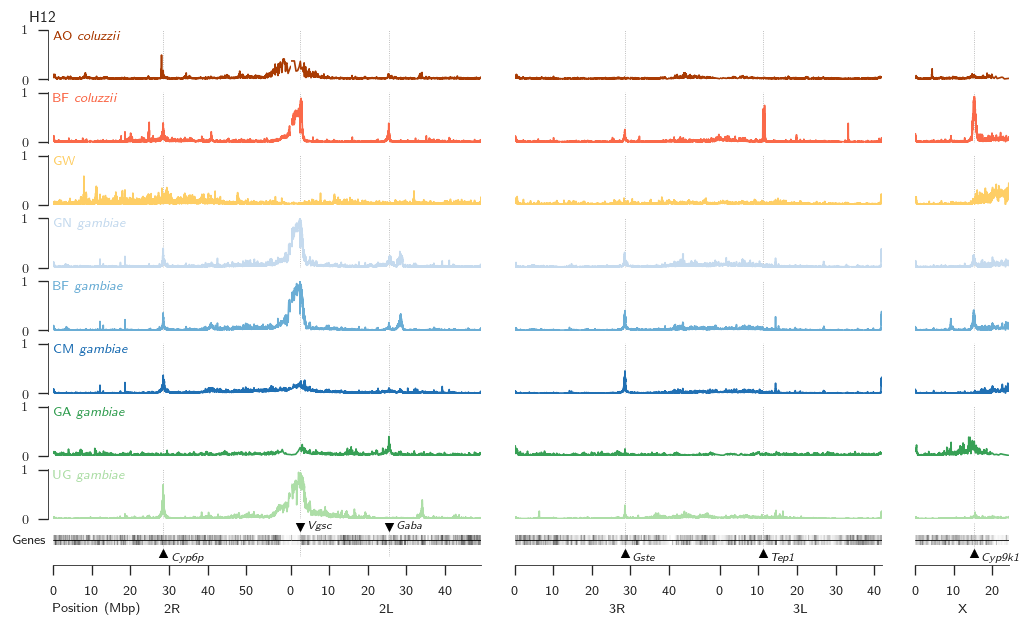
\includegraphics[width=1.1\textwidth,center]{artwork/chapter5/h12.png}
\caption{H12 selection scans.
%
Each track shows results from H12 selection scan in a single population.
%
AO = Angola; BF = Burkina Faso; GW = Guinea-Bissau; GN = Guinea; CM = Cameroon; GA = Gabon; UG = Uganda.
%
H12 values range between 0 and 1, where a value of zero indicates high haplotype diversity within a genomic window, and a value of one indicates low haplotype diversity (at most two distinct haplotypes observed within the sampled individuals).
%
Validated insecticide resistance genes (\textit{Vgsc}, \textit{Gaba}, \textit{Cyp9k1}) or gene clusters (\textit{Cyp6p}, \textit{Gste}) are labelled at the bottom.
%
\textit{Tep1} is an immune system gene previously found to be under selection in \acol~\parencite{White2011}.
% @@TODO stretch this figure!
}
\label{fig:h12}
\end{figure}


To provide an initial view of these data, I plotted the results of the H12 scans over the genome (Fig.~\ref{fig:h12}).
%
There were a number of clear peaks within these scans that were replicated across multiple populations, including at the following five loci containing genes that have been functionally validated as playing a role in insecticide resistance in \agam\ and/or \acol:
%
\begin{itemize}
%%
\item \textbf{2L:2.4 Mb} - This locus contains the voltage-gated sodium channel gene (\textit{Vgsc}; \texttt{AGAP004707}) which encodes a nervous system protein that is the binding target of DDT and pyrethroid insecticides~\parencite{Dong2014}.
%
Amino acid substitutions in this gene confer resistance to DDT and pyrethroids in \agam~\parencite{MartinezTorres1998,Ranson2000a,Davies2007,Lynd2010,Jones2012,Wang2015}.
%%
\item \textbf{3R:28.6 Mb} - This locus contains a cluster of eight glutathione S-transferase genes, which encode enzymes involved in detoxification of xenobiotic substances.
%
In \agam\ this locus was initially discovered as a major locus of DDT resistance~\parencite{Prapanthadara1993,Ranson2000b,Ranson2001,Ding2003}.
%
An amino acid substitution in one of the genes in this cluster, \textit{Gste2} (\texttt{AGAP009194}) was subsequently shown to confer elevated DDT resistance~\parencite{Mitchell2014}.
%
Increased expression of \textit{Gste2} has also been shown experimentally to confer resistance to DDT and organophosphates~\parencite{Adolfi2019}.
%%
\item \textbf{2R:28.5 Mb} - This locus contains a cluster of ten genes, nine of which encode cytochrome P450 enzymes.
%
This includes \textit{Cyp6p3} (\texttt{AGAP002865}) which is associated with pyrethroid resistance in \agam\ and is capable of metabolising multiple pyrethroid insecticides~\parencite{Muller2008}.
%
Increased expression of \textit{Cyp6p3} has also been shown experimentally to confer resistance to both pyrethroids and carbamates in \agam~\parencite{Adolfi2019}.
%%
\item \textbf{X:15.2 Mb} - This locus contains the cytochrome P450 gene \textit{Cyp9k1} (\texttt{AGAP000818}).
%
A selection signal has previously been found at this locus in \acol\ in Mali~\parencite{Main2015}.
%
Evolution of \textit{Cyp9k1} has also been observed in \acol\ on Bioko Island in response to combined use of pyrethroids in IRS and LLIN programmes~\parencite{Vontas2018}.
%
\textit{Cyp9k1} metabolises the pyrethroid deltamethrin, but also pyriproxyfen, a non-pyrethroid insecticide~\parencite{Vontas2018}.
%%
\item \textbf{2L:25.4 Mb} - This locus contains the \textit{Gaba} gene (\texttt{AGAP006028}) and is also known as the resistance to dieldrin (\textit{Rdl}) locus.
%
This gene encodes another component of the nervous system,  the gamma-aminobutyric acid receptor subunit, which is the binding target for the insecticide dieldrin.
%
Dieldrin use ceased in the 1970s, but resistance has remained persistent in \textit{Anopheles} for decades afterwards~\parencite{Du2005}.
%
Amino acid substitutions are known in \agam\ and \acol\ to confer dieldrin resistance~\parencite{Du2005,Lawniczak2010}.
\end{itemize}


Although these five loci contain genes with a known role in insecticide resistance, the fact that there are strong signals of selection in multiple populations in the Ag1000g phase 1 cohort provides valuable confirmation that these loci are indeed playing an important role in adaptation to insecticide pressure in natural malaria vector populations.
%
Because we have a strong prior expectation for selection at these loci, they also provide us with valuable positive controls, allowing us to study the character of true selection signals in more detail.
%
This in turn can guide the design and calibration of algorithms for discovering signals of selection for insecticide resistance at novel loci.


%%%%%%%%%%%%%%%%%%%%%%%%%%%%%%%%%%%%%%%%%%%%%%%%%%%%%%%%%%%%%%%%%%%%%%%%%%%%%%%
%%%%%%%%%%%%%%%%%%%%%%%%%%%%%%%%%%%%%%%%%%%%%%%%%%%%%%%%%%%%%%%%%%%%%%%%%%%%%%%
\subsection{Selection signal discovery and mapping}\label{subsec:signal-discovery}


\begin{figure}[t!]
    \centering
    \begin{subfigure}[t]{0.32\textwidth}
        \centering
        \caption{}
        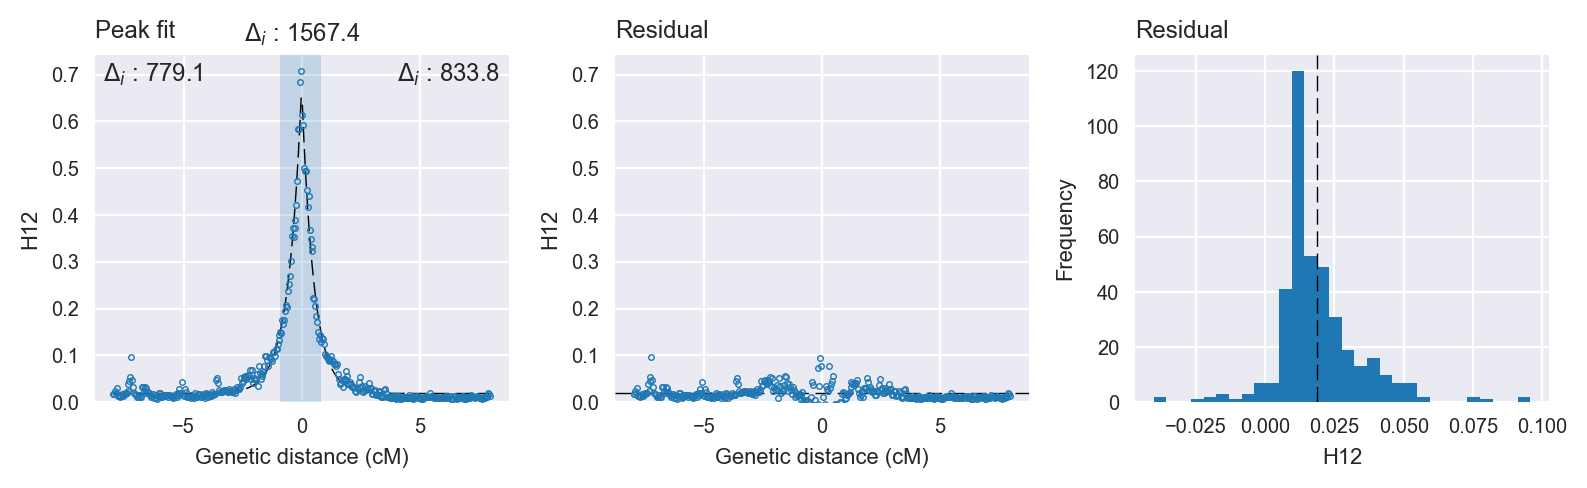
\includegraphics[width=1.1\textwidth,center,trim=0 27 380 0, clip]{artwork/chapter5/peak_fit_h12_cyp6p_ugs.png}
    \end{subfigure}
    \hfill
    \begin{subfigure}[t]{0.32\textwidth}
        \centering
        \caption{}
        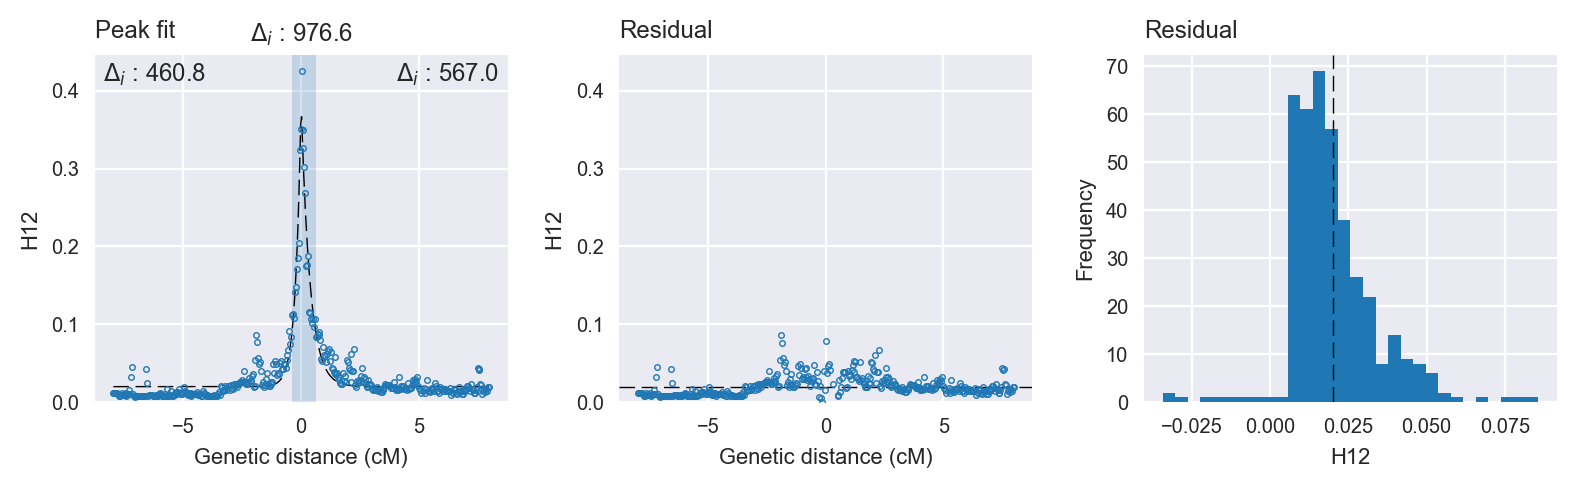
\includegraphics[width=1.1\textwidth,center,trim=0 27 380 0, clip]{artwork/chapter5/peak_fit_h12_cyp6p_bfs.png}
    \end{subfigure}
    \hfill
    \begin{subfigure}[t]{0.32\textwidth}
        \centering
        \caption{}
        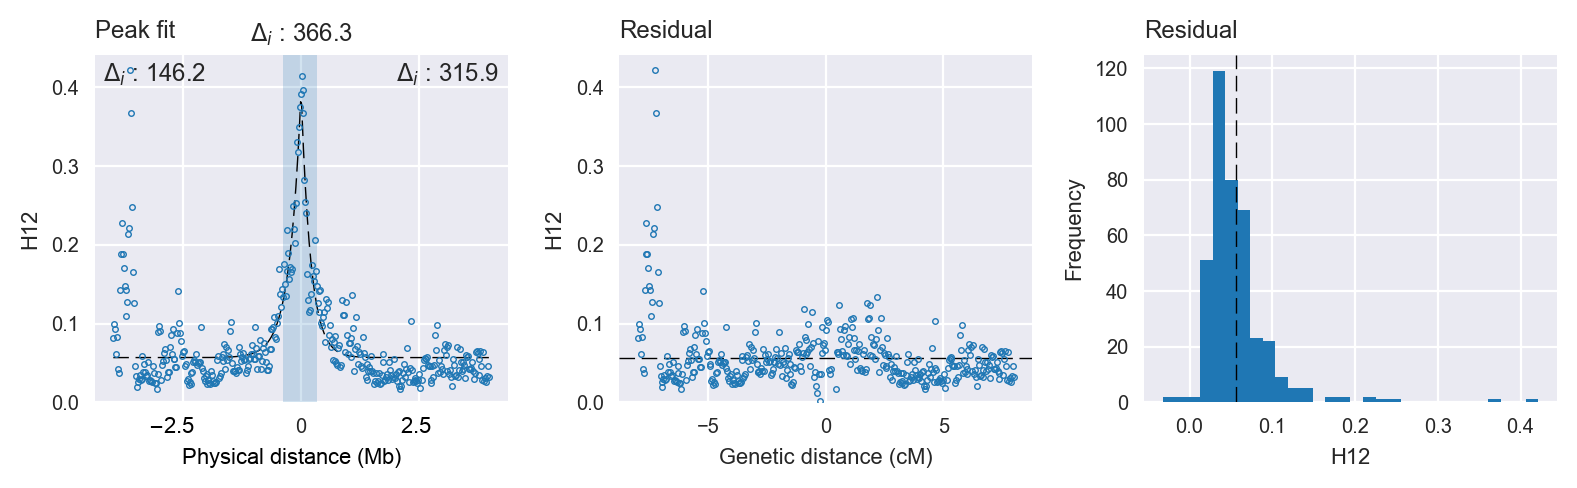
\includegraphics[width=1.1\textwidth,center,trim=0 27 380 0, clip]{artwork/chapter5/peak_fit_h12_cyp6p_bfm.png}
    \end{subfigure}
    \vspace{0cm}
    \begin{subfigure}[t]{0.32\textwidth}
        \centering
        \caption{}
        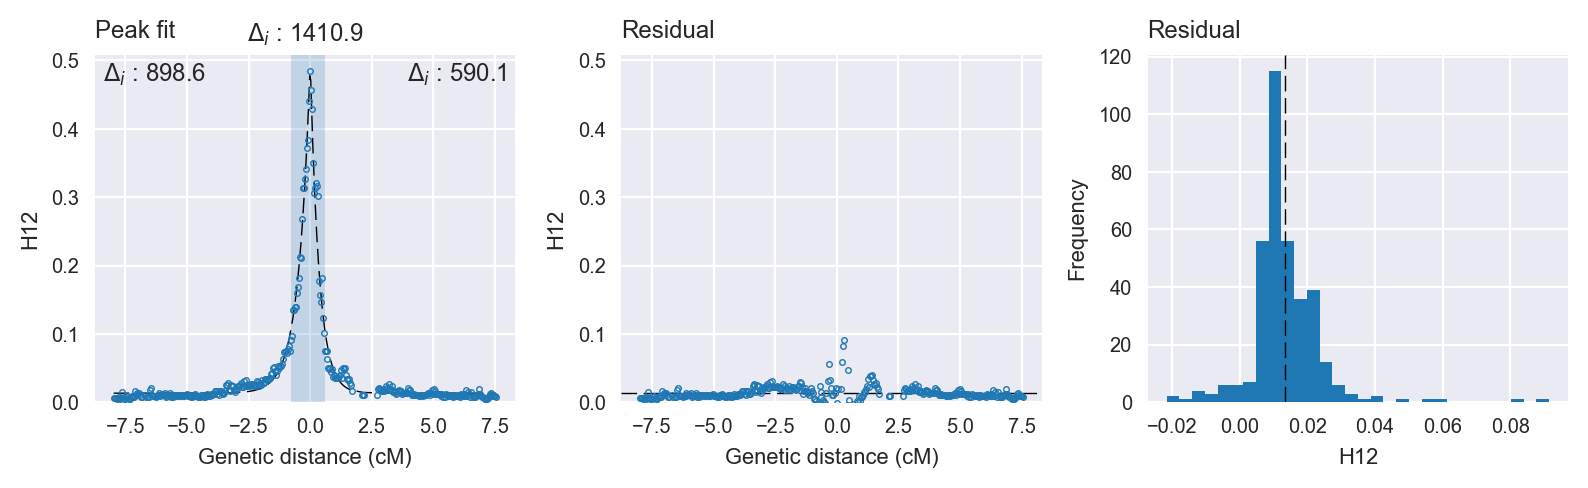
\includegraphics[width=1.1\textwidth,center,trim=0 27 380 0, clip]{artwork/chapter5/peak_fit_h12_gste_cms.png}
    \end{subfigure}
    \hfill
    \begin{subfigure}[t]{0.32\textwidth}
        \centering
        \caption{}
        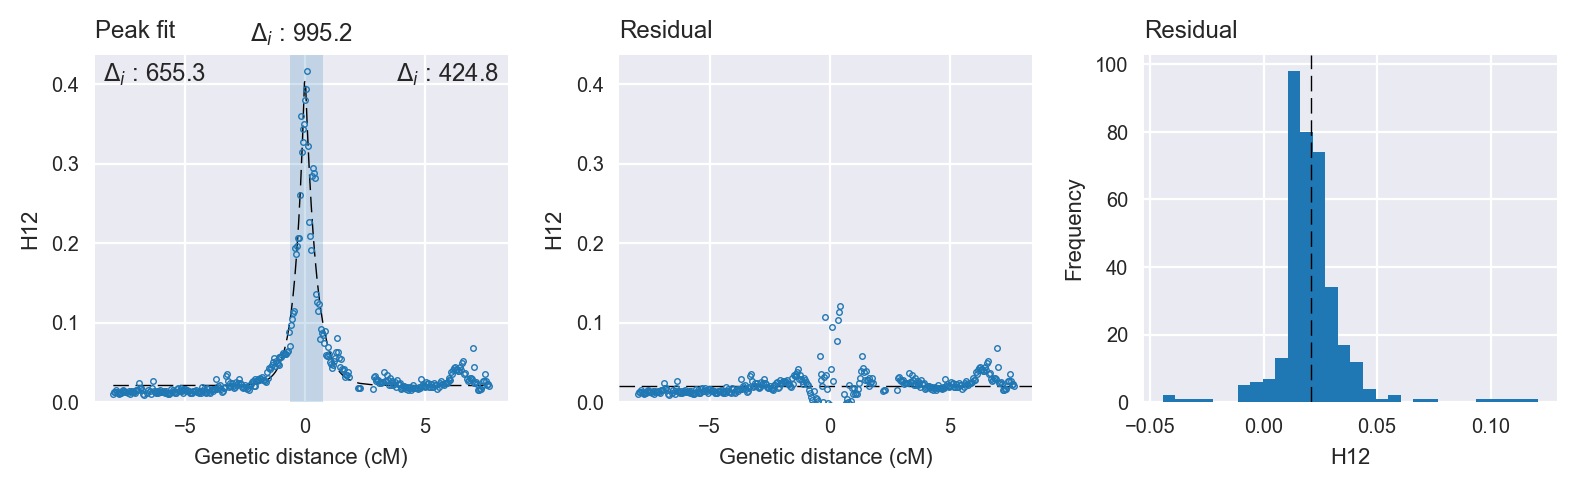
\includegraphics[width=1.1\textwidth,center,trim=0 27 380 0, clip]{artwork/chapter5/peak_fit_h12_gste_bfs.png}
    \end{subfigure}
    \begin{subfigure}[t]{0.32\textwidth}
        \centering
        \caption{}
        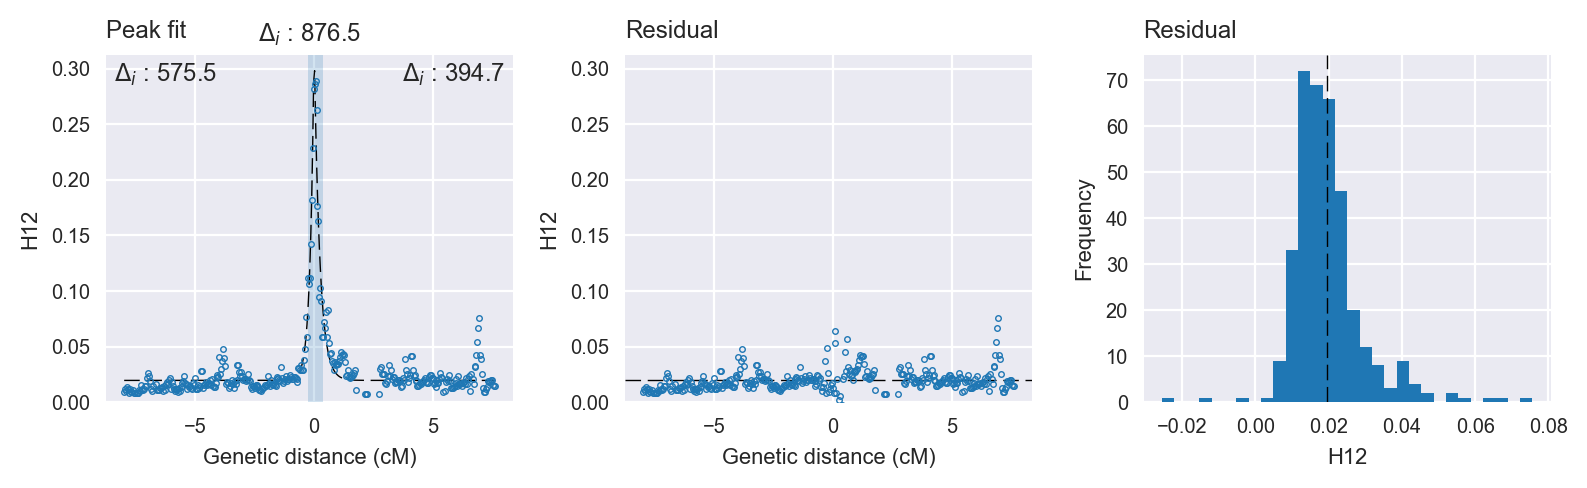
\includegraphics[width=1.1\textwidth,center,trim=0 27 380 0, clip]{artwork/chapter5/peak_fit_h12_gste_ugs.png}
    \end{subfigure}
    \vspace{0cm}
    \begin{subfigure}[t]{0.32\textwidth}
        \centering
        \caption{}
        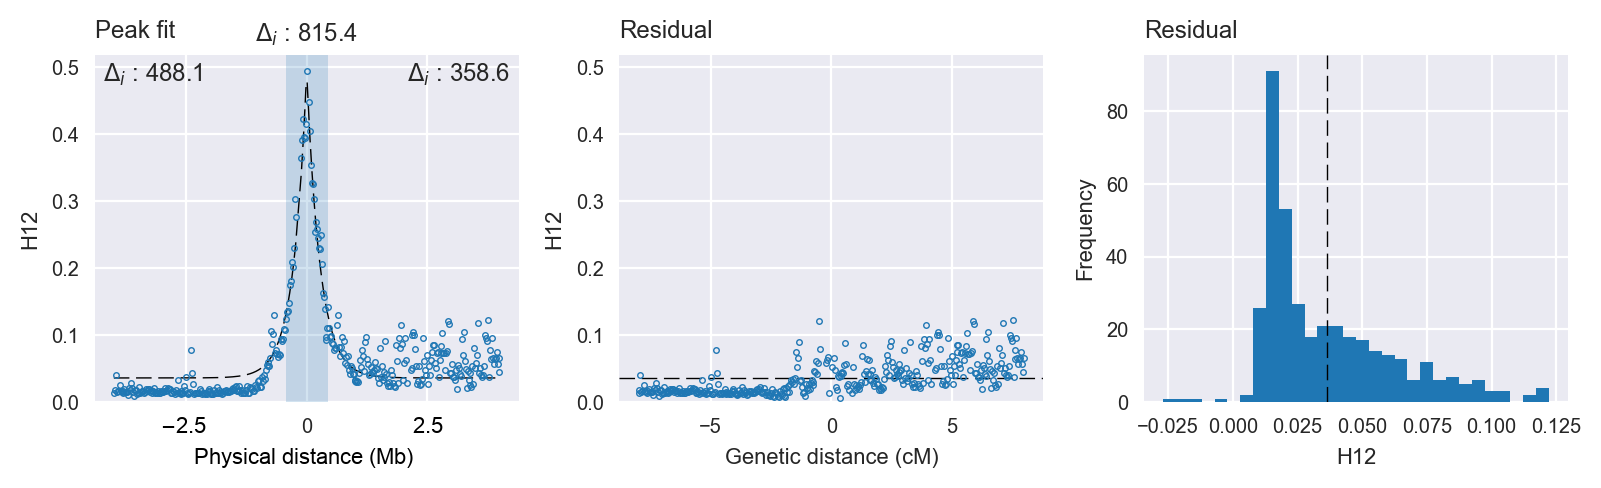
\includegraphics[width=1.1\textwidth,center,trim=0 27 380 0, clip]{artwork/chapter5/peak_fit_h12_cyp9k1_bfs.png}
    \end{subfigure}
    \hfill
    \begin{subfigure}[t]{0.32\textwidth}
        \centering
        \caption{}
        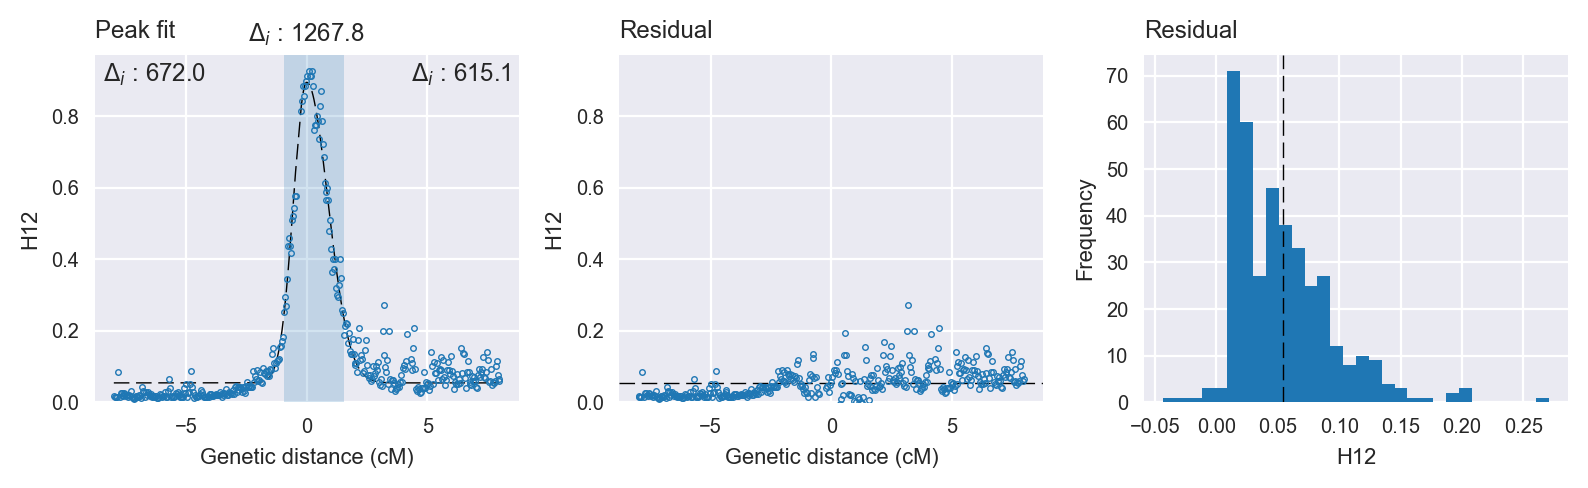
\includegraphics[width=1.1\textwidth,center,trim=0 27 380 0, clip]{artwork/chapter5/peak_fit_h12_cyp9k1_bfm.png}
    \end{subfigure}
    \begin{subfigure}[t]{0.32\textwidth}
        \centering
        \caption{}
        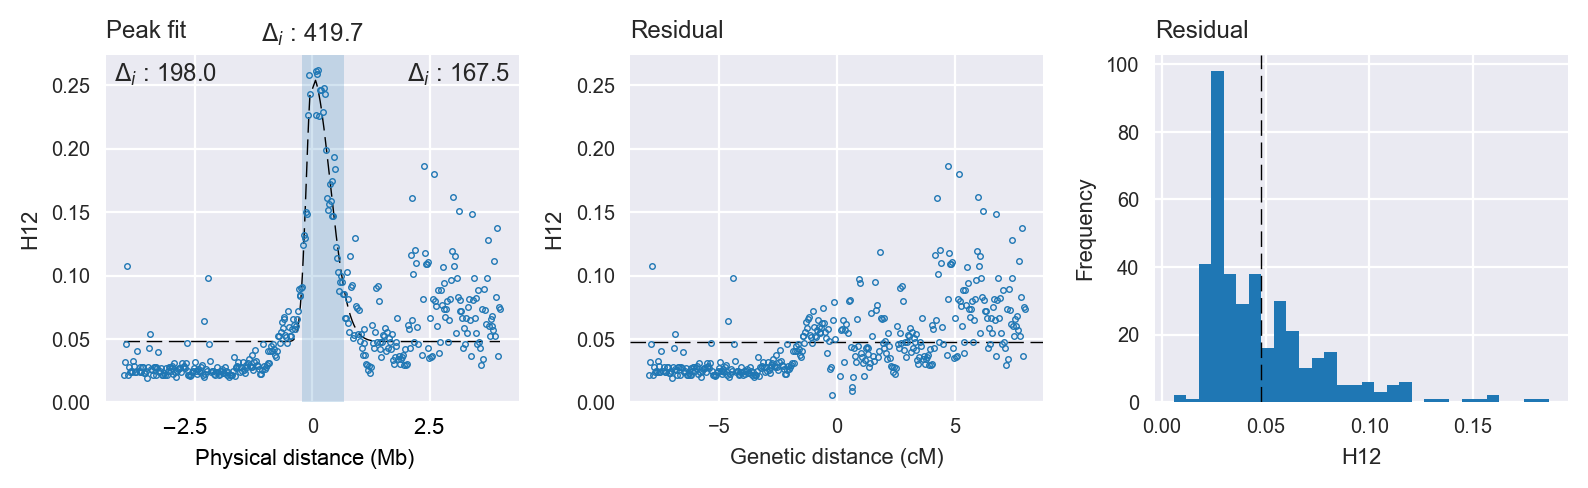
\includegraphics[width=1.1\textwidth,center,trim=0 27 380 0, clip]{artwork/chapter5/peak_fit_h12_cyp9k1_gns.png}
    \end{subfigure}
    \vspace{0cm}
    \begin{subfigure}[t]{0.32\textwidth}
        \centering
        \caption{}
        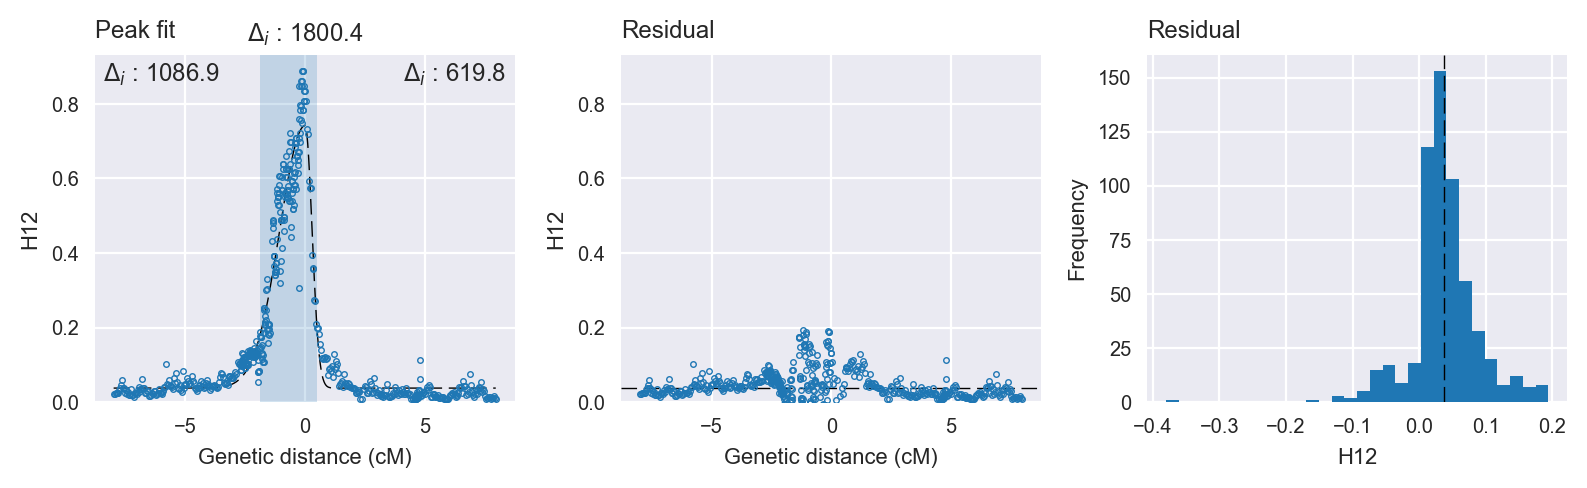
\includegraphics[width=1.1\textwidth,center,trim=0 0 380 0, clip]{artwork/chapter5/peak_fit_h12_vgsc_bfm.png}
    \end{subfigure}
    \hfill
    \begin{subfigure}[t]{0.32\textwidth}
        \centering
        \caption{}
        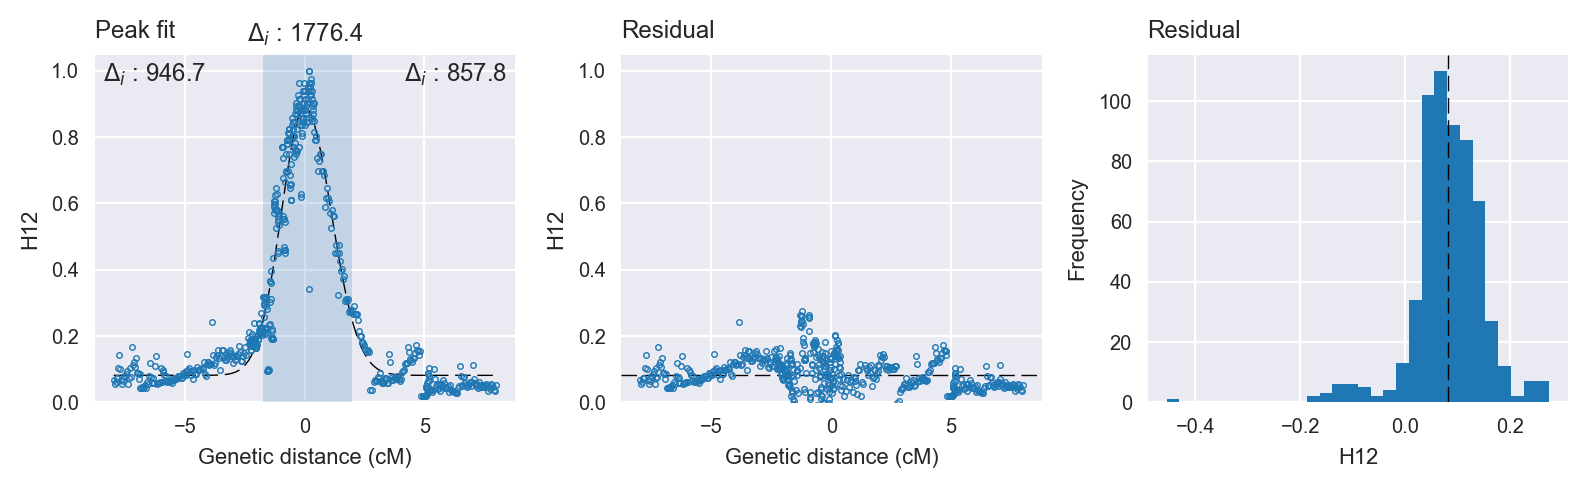
\includegraphics[width=1.1\textwidth,center,trim=0 0 380 0, clip]{artwork/chapter5/peak_fit_h12_vgsc_bfs.png}
    \end{subfigure}
    \begin{subfigure}[t]{0.32\textwidth}
        \centering
        \caption{}
        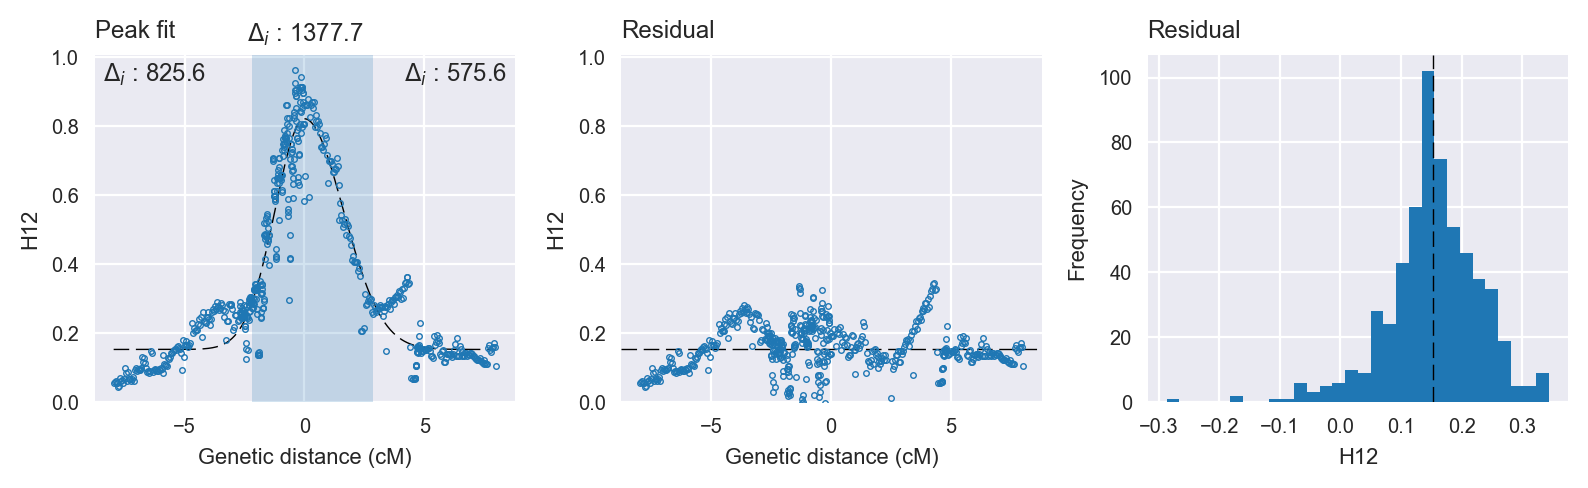
\includegraphics[width=1.1\textwidth,center,trim=0 0 380 0, clip]{artwork/chapter5/peak_fit_h12_vgsc_ugs.png}
    \end{subfigure}
    \caption{Examples of peak models fitted to H12 selection scans at known insecticide resistance loci using least-squares regression. Dashed lines show model fit, markers show data. \textbf{a}, \textit{Cyp6p}, Uganda \agam. \textbf{b}, \textit{Cyp6p}, Burkina Faso \agam. \textbf{c}, \textit{Cyp6p}, Burkina Faso \acol. \textbf{d}, \textit{Gste}, Cameroon \agam. \textbf{e}, \textit{Gste}, Burkina Faso \agam. \textbf{f}, \textit{Gste}, Uganda \agam. \textbf{g}, \textit{Cyp9k1}, Burkina Faso \agam. \textbf{h}, \textit{Cpy9k1}, Burkina Faso \acol. \textit{i}, \textit{Cyp9k1, Guinea \agam}. \textbf{j}, \textit{Vgsc}, Burkina Faso \acol. \textbf{k}, \textit{Vgsc}, Burkina Faso \agam. \textbf{l}, \textit{Vgsc}, Uganda \agam.}
    \label{fig:peak_fits}
\end{figure}


To learn more about the character of signals of selection for insecticide resistance, I studied the selection scan statistics in more detail at the five known insecticide resistance loci listed above.
%
A common feature of selection signals at these loci was a clear peak architecture, with a maximum (peak) value close to the target gene, and values of the selection statistic decaying to background levels both upstream and downstream of the gene.
%
In the H12 selection scans in particular, values on either side of the target gene appeared to decay asymptotically, and it occurred to me to model this decay by fitting exponential functions to each flank of a selection signal via least-squares regression.
%
This exponential peak model provided a good fit to the selection signals at many of the known insecticide resistance loci (e.g., Fig.~\ref{fig:peak_fits}a-g).
%
I also tested several other peak models, and found that a Gaussian peak model provided a better fit in a minority of cases (e.g., Fig.~\ref{fig:peak_fits}h-l).
%
At the \textit{Vgsc} locus the peaks were highly skewed when plotted against physical genome coordinates, but this locus lies on the border of pericentromeric heterochromatin, and this skew could be almost entirely corrected by assuming the heterochromatin recombination rate is four times lower than euchromatin.
%
I devised a way to quantify the support for these peak models by also fitting a null constant model at the same locus and computing the difference in Akaike Information Criterion ($\Delta_i$) between the peak and null models.
%
In general, when comparing two models, $\Delta_i > 10$ is considered sufficient evidence to reject the model with higher AIC~\parencite{Burnham2002}, and at many of the known insecticide resistance loci I observed $\Delta_i > 1000$, indicating strong support for the exponential peak model.
%


Previous studies performing genome-wide selection scans, such as \textcite{Garud2015}, have identified peaks by first choosing a fixed significance threshold, and then defining peaks to be contiguous genome regions where selection scan values exceed this threshold.
%
Such an approach, however, can have several shortcomings, illustrated in the Ag1000G data in Fig.~\ref{fig:peak_problems}.
%
Firstly, determining an appropriate significance threshold is not straightforward, and requires knowledge of the demographic history of the population being studied, which may be unknown or difficult to infer with any certainty.
%
Secondly, different types of noise within the data can lead to incorrect inferences, such as mistakenly inferring a signal from an isolated high statistic value, or mistakenly splitting a peak into two signals due to an isolated low statistic value.
%
Thirdly, from inspecting another known insecticide resistance gene, \textit{Ace1} (\texttt{AGAP001356}), it was also clear that signals might be small in magnitude despite having a clear peak architecture, and so fall below a fixed significance threshold.
%
Examining the Ag1000G selection scans at known insecticide resistance loci suggests how these issues could be overcome by leveraging the information provided by the shape of peaks at true selection signals.
%
At a locus under recent positive selection, genetic hitchhiking of neutral variants on either flank of the locus is expected due to linkage disequilibrium, and the probability of linkage is an exponential function of the genetic distance between them~\parencite{MaynardSmith1974}.
%
\textcite{Wiener2011} showed that this theory could be used as a tool for mapping selection signals, by fitting exponential functions to heterozygosity data on either flank of a locus under positive selection via least squares regression.
%
The primary benefit of this type of approach to modelling support for a selection signal is that it integrates evidence not just at the locus under selection, but from the flanking regions as well.
%


\begin{figure}[t!]
\centering
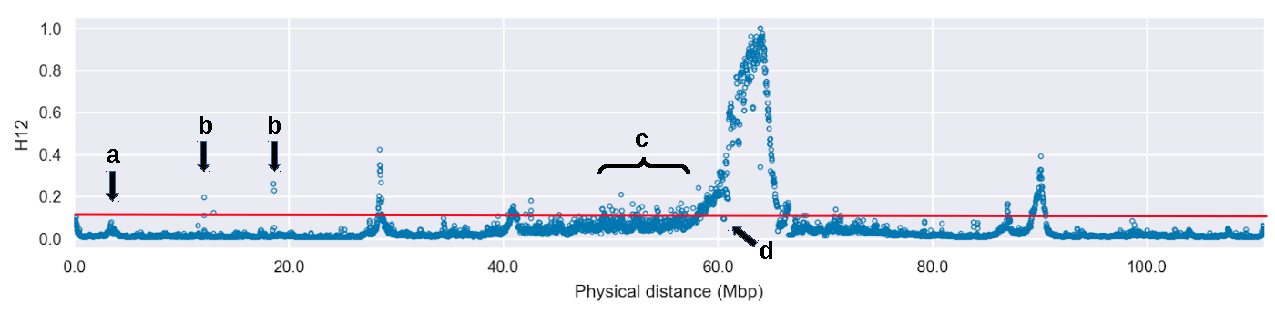
\includegraphics[width=1.1\textwidth,center]{artwork/chapter5/peak_problems.pdf}
\caption{Illustration of potential problems with peak identification using consecutive windows exceeding a fixed threshold, as applied by \textcite{Garud2015}.
%
Blue markers show H12 values from selection scan in Burkina Faso \agam.
%
Red line shows an arbitrary significance threshold, chosen to illustrate potential problems in these data (these problems are associated with the use of a fixed threshold and can arise regardless of the actual threshold value chosen).
%
\textbf{a}, This locus contains the known insecticide resistance gene \textit{Ace1}, and a small peak is visible in the selection scan, but the magnitude of the peak falls below the threshold and so would not be discovered.
%
\textbf{b}, Isolated high values of the selection statistic are probably false positives due to noise, such signals are never observed at known insecticide resistance genes.
%
\textbf{c}, Some genome regions can be inherently noisier than others, i.e., background levels of the selection statistic are higher.
%
\textbf{d}, Isolated low values of the selection statistic could falsely lead us to break up a single peak into two peaks, such as at this selection signal at the \textit{Vgsc} insecticide resistance gene.
}
\label{fig:peak_problems}
\end{figure}


Developing this idea further, I devised an algorithm to systematically identify selection signals within each of the Ag1000G selection scans, quantify their support, map the most likely focus of selection, and provide some indication of the relative uncertainty surrounding the mapped focus.
%
The algorithm uses non-linear least squares regression to fit peak and null models to the selection scan values at regular 20 kb intervals throughout the genome.
%
After performing a complete scan through the genome, the peak model with the highest $\Delta_i$ is called as a signal.
%
To deal with cases where true selection signals occur in close proximity and peaks may be partially overlapping, the algorithm then subtracts the fitted peak values from the data, and refits peaks in adjacent regions.
%
This process is then applied iteratively, until no more peak models with $\Delta_i$ above a given level are found.
%
After applying this algorithm to all Ag1000G selection scans, I found all peaks overlapping known insecticide resistance genes had $\Delta_i > 90$, and so only called signals above this level.
%
This generated a catalog of 289 selection signals (Figs.~\ref{fig:signals_2R},~\ref{fig:signals_2L},~\ref{fig:signals_3R},~\ref{fig:signals_3L},~\ref{fig:signals_X}), which I then ranked by $\Delta_i$.
%


%%%%%%%%%%%%%%%%%%%%%%%%%%%%%%%%%%%%%%%%%%%%%%%%%%%%%%%%%%%%%%%%%%%%%%%%%%%%%%%
%%%%%%%%%%%%%%%%%%%%%%%%%%%%%%%%%%%%%%%%%%%%%%%%%%%%%%%%%%%%%%%%%%%%%%%%%%%%%%%
\subsection{Signal discovery and mapping performance}\label{subsec:performance}


To provide some assessment of the performance of the signal discovery algorithm, I took an empirical approach, making use of the five known insecticide resistance genes described above, in addition to the \textit{Ace1} gene where variants are known to confer resistance to carbamate and organophosphate insecticides~\parencite{Weill2003,Weill2004,Djogbenou2008}.


To estimate sensitivity I analysed the \textit{Vgsc}, \textit{Gaba}, \textit{Ace1} and \textit{Gste2} genes, where SNPs conferring insecticide resistance are known from previous studies.
%
For each of these genes I ascertained the populations in which a known resistance variant was at 5\% allele frequency or greater, and used these as a truth set.
%
I then determined a true positive to be a population in which a selection signal was found overlapping the gene, and a false negative to be a population in which no overlapping selection signal was found.
%
Across all four loci and three selection scan methods, the overall sensitivity was 100\% (Table~\ref{table:sens}).
%
Sensitivity was highest in the H12 and XPEHH scans (both 79\%) and lowest in the IHS scans (37\%).
%


To estimate signal mapping accuracy I used all six known insecticide resistance genes.
%
For each selection signal overlapping one of these genes, I computed the mapping error (ME) as the distance from the fitted peak centre to the gene center, then summarised these values across multiple scans and loci by computing the median and $25-75^{th}$ percentiles (Table~\ref{table:acc}).
%
Across all six loci, median mapping error was lowest in the H12 scans (78 kb) and highest in the IHS scans (258 kb).
%
To estimate a confidence interval for the focus of selection within each peak I computed the region within which peak models obtained $\Delta_i$ within 95\% of the best peak model.
%
This confidence interval was correlated with the mapping error in the H12 and XPEHH signals but not IHS (Fig.~\ref{fig:accuracy}).
%
This confidence included the target gene in 33--63 \% of cases depending on scanning method, and increased to 56--68 \% if extended by 50 kb.
%
Clearly there is room for improvement here in estimating a confidence interval for the focus of the selection signal, but at least for the H12 and XPEHH scans there is an indication that some uncertainty is being captured.


%%%%%%%%%%%%%%%%%%%%%%%%%%%%%%%%%%%%%%%%%%%%%%%%%%%%%%%%%%%%%%%%%%%%%%%%%%%%%%%
%%%%%%%%%%%%%%%%%%%%%%%%%%%%%%%%%%%%%%%%%%%%%%%%%%%%%%%%%%%%%%%%%%%%%%%%%%%%%%%
\subsection{A Web application for exploring selection signals}\label{subsec:webapp}


Of the 289 selection signals identified, 229 did not overlap any of the known insecticide resistance loci described above.
%
To facilitate an exploration of these potentially novel selection signals, and an investigation of the genes that might be driving them, I developed a prototype Web application, available at \url{https://malariagen.github.io/agam-selection-atlas/}.
%
Each selection signal can span multiple genes, and thus it can be time-consuming to explore signals and generate hypotheses about the most likely candidate genes under selection.
%
The purpose of the Web application is to accelerate this investigation process, by providing a visual interface to the data, with tools for comparing selection signals across populations and selection scans, and for zooming into individual signals and inspecting genes.
%
The Web application provides several entry points to the data, including:
%
\begin{itemize}
    %
    \item \textbf{All selection signals}.
    %
    A table of selection signals, ranked by the degree of supporting evidence ($\Delta_i$).
    %
    For each signal, the table provides the selection statistic, the population in which the signal was found, the focal region, and whether the signal overlaps any known loci.
    %
    \item \textbf{Signals by population}.
    %
    One page for each population, with an interactive genome plot for each chromosome arm providing a means to view and browse the selection signals, and an associated table of selection signals.
    %
    \item \textbf{Signals by chromosome arm}.
    %
    One page for each chromosome arm, with an interactive genome plot showing signals from all populations, and an associated table of signals (Figs.~\ref{fig:signals_2R},~\ref{fig:signals_2L},~\ref{fig:signals_3R},~\ref{fig:signals_3L} and~\ref{fig:signals_X} are screenshots from these pages).
    %
    \item \textbf{Signals by scanning statistic}.
    %
    One page for each scanning method used (H12, XPEHH, IHS), with a table of associated selection signals from all populations and chromosome arms.
    %
    \item \textbf{Known loci}.
    %
    A set of pages for functionally-validated insecticide resistance loci where there is a strong expectation for observing selection signals in at least some populations.
    %
    \item \textbf{Insecticide resistance candidate genes}.
    %
    Pages providing catalogues of \textit{a priori} candidate insecticide resistance genes based on gene function, organised into four lists: metabolic, target-site, behavioural and cuticular.
\end{itemize}


From these entry points, a user can access a dedicated \textbf{signal page} for each individual selection signal.
%
Each signal page includes an interactive genome plot for the region containing and surrounding the peak, showing the selection statistic values, and the fitted peak model (Fig.~\ref{fig:dgk} panels a-d are screenshots of this feature from four signal pages).
%
This plot can be zoomed and panned to allow inspection of the genes nearest to the peak centre.
%
The set of genes overlapping the inferred focal region are also listed below the plot.
%
There is also a table of overlapping selection signals, which can be useful to assess the degree of replication across both populations and selection methods.
%
Finally, there are a collection of diagnostic plots, and a model fit report, providing detailed information to allow assessment of how well the peak model fitted the data.
%
If a user wants to investigate a particular gene of interested, then can click through to a dedicated \textbf{gene page}.
%
Each gene page as summary information about the gene, with links through to VectorBase, and a table of all overlapping and adjacent selection signals.



%%%%%%%%%%%%%%%%%%%%%%%%%%%%%%%%%%%%%%%%%%%%%%%%%%%%%%%%%%%%%%%%%%%%%%%%%%%%%%%
%%%%%%%%%%%%%%%%%%%%%%%%%%%%%%%%%%%%%%%%%%%%%%%%%%%%%%%%%%%%%%%%%%%%%%%%%%%%%%%
\subsection{Discovery of a novel candidate insecticide resistance gene}\label{subsec:novel}


\begin{figure}[t!]
\centering
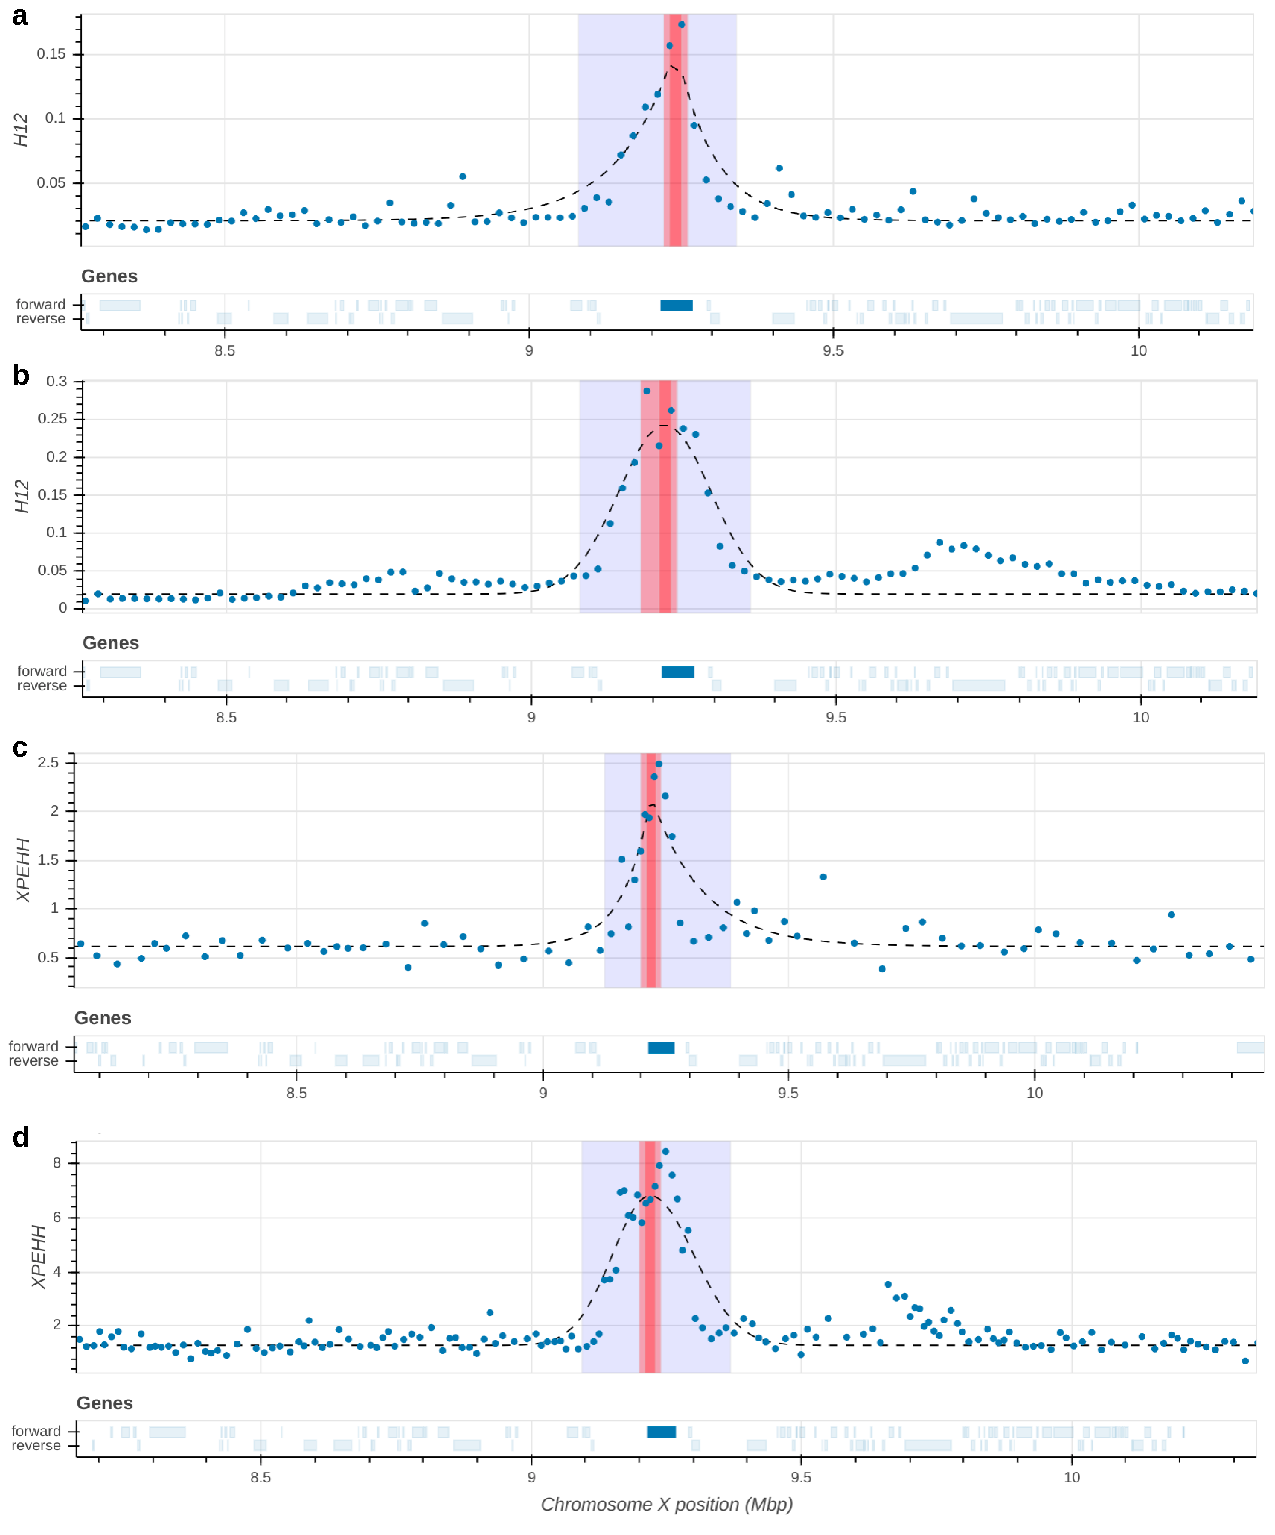
\includegraphics[width=1\textwidth,center]{artwork/chapter5/dgk.pdf}
\caption{Selection signals at a novel locus on the X chromosome.
%
The gene shown in blue in all subplots is \texttt{AGAP000519}, a diacylglycerol kinase.
%
\textbf{a}, Burkina Faso \acol, H12.
%
\textbf{b}, Burkina Faso \agam, H12.
%
\textbf{c}, Burkina Faso \acol, XPEHH versus Guinea-Bissau.
%
\textbf{d}, Burkina Faso \agam, XPEHH versus Guinea-Bissau.
}
\label{fig:dgk}
\end{figure}


To illustrate the potential of these selection scans to identify novel candidate insecticide resistance genes, I provide an example of selection signals at a novel locus on the X chromosome (Fig.~\ref{fig:dgk}).
%
Selection signals were found at this locus in both species from Burkina Faso, and were replicated in both populations across all three selection scan methods.
%
Selection peaks were also relatively narrow, and only a single gene overlapped the peak focus in all H12 and XPEHH scans.
%
This gene was \texttt{AGAP000519}, a diacylglycerol kinase.
%
This gene is intriguing because its function does not obviously fit any of the established categories of insecticide resistance gene.
%
I performed a literature search and could not find any previous studies associating diacylglycerol kinase enzymes with insecticide resistance in any insect species.
%
I did, however, find two lines of evidence suggesting a potential role in adaptation to malaria vector control interventions.


In \textit{C. elegans}, the diacylglycerol kinase DGK-1 is involved in regulating release of the neurotransmitter acetylcholine at synaptic junctions~\parencite{Miller1999}.
%
This discovery was made by using genetic screens for mutants with resistance to aldicarb, a carbamate insecticide.
%
Carbamates bind to acetylcholinesterase and prevent its normal function in inactivating acetylcholine, causing a toxic accumulation of acetylcholine at synapses.
%
Mutations in the upstream regulatory pathway that reduce the normal amount of acetylcholine present in synapses can thus alter sensitivity to carbamates.
%
\textcite{Miller1999} found mutations in several genes that confer aldicarb resistance by this means.
%
They also found that DGK-1 is a component of this regulatory machinery, and normally acts to negatively regulate synaptic transmission.
%
A loss of function in DGK-1 results in hypersensitivity to aldicarb, in addition to hyperactive locomotion.
%
If synaptic transmission is regulated via a similar pathway in \textit{Anopheles} mosquitoes, then this suggests a hypothesis that a gain of function mutation in a diacylglycerol kinase gene could confer some degree of resistance to carbamate and organophosphate insecticides, which share the same mode of action.
%
Carbamates have been used for indoor residual spraying (IRS) fairly extensively, and organophosphates are increasingly being used, thus any novel mechanism of resistance to these insecticides in malaria vectors would be of high importance.


There is also a second hypothesis, concerning a possible role in behavioural adaptation.
%
\texttt{AGAP000519} is a one-to-one homolog of the \textit{D. melanogaster} gene \textit{rdgA}.
%
In \textit{D. melanogaster}, \textit{rdgA} is an eye-specific diacylglycerol kinase involved in vision via the phototransduction signalling cascade~\parencite{Masai1993}.
%
\textit{rdgA} loss-of-function mutants have constitutive activation of light-sensitive ion channels, causing retinal degeneration during development~\parencite{Raghu2000}.
%
These observations have demonstrated that \textit{rdgA} is required for light signalling response termination via the phosphoinositide cycle~\parencite{Katz2009}.
%
Thus, any modulation of the activity of \textit{rdgA} has the potential to affect sensitivity to light.
%
In \agam, genes in this visual signalling pathway, including \texttt{AGAP000519}, are expressed rhythmically under circadian clock control~\parencite{Rund2011}.
%
Expression peaks just before dusk, suggesting a role in tuning the \agam\ visual system ahead of nocturnal activities such as flight and biting.
%
The increase in coverage of insecticide-treated bednets has long been hypothesised to create a selective pressure for individuals that initiate host-seeking behaviour earlier in the night, but no genetic changes have so far been found affecting this behaviour.
%


Diacylglycerol is a signalling molecule used in a variety of other roles, and there may be other causes for selection at this locus in \agam\ and \acol.
%
Nevertheless, the presence of clear selection signals at this locus in both species, the high degree of confidence regarding the target gene, and the presence of compelling and plausible links to adaptation to vector control interventions, strongly advise for the further study of this gene.
%
Furthermore, although the two hypotheses presented above are different, the underlying molecular pathways are the same on both cases, with diacylglycerol kinase enzymes serving to modulate the excitability of neurons.
%
This in turn argues for a deeper study of this pathway in malaria vectors.


%%%%%%%%%%%%%%%%%%%%%%%%%%%%%%%%%%%%%%%%%%%%%%%%%%%%%%%%%%%%%%%%%%%%%%%%%%%%%%%
%%%%%%%%%%%%%%%%%%%%%%%%%%%%%%%%%%%%%%%%%%%%%%%%%%%%%%%%%%%%%%%%%%%%%%%%%%%%%%%
%%%%%%%%%%%%%%%%%%%%%%%%%%%%%%%%%%%%%%%%%%%%%%%%%%%%%%%%%%%%%%%%%%%%%%%%%%%%%%%
\section{Conclusions}\label{sec:ch5-conclusions}


In this chapter I have explored the genomic landscape of recent selection within the mosquito populations sampled in the first phase of the Ag1000G project.
%
There are strong signals of selection at multiple loci with clear links to insecticide resistance, demonstrating that malaria vector control interventions have driven a strong adaptive response.
%
It is also clear that this adaptive response is both polygenic and heterogeneous over both species and geography, with different genes under selection in different combinations of populations.
%
Furthermore, a substantial number of selection signals are present at genes not previously known to be involved in insecticide resistance, where signals are of comparable shape and statistical support to those found at validated insecticide resistance genes.
%
This strongly suggests that the molecular landscape of insecticide resistance in \agam\ and \acol\ is not fully understood and there are major gaps in our current knowledge.
%
The Ag1000G data provide a unique opportunity to fill some of these gaps, generating new candidate genes under selection for further investigation and validation through lab and field work.


%%%%%%%%%%%%%%%%%%%%%%%%%%%%%%%%%%%%%%%%%%%%%%%%%%%%%%%%%%%%%%%%%%%%%%%%%%%%%%%
%%%%%%%%%%%%%%%%%%%%%%%%%%%%%%%%%%%%%%%%%%%%%%%%%%%%%%%%%%%%%%%%%%%%%%%%%%%%%%%
%%%%%%%%%%%%%%%%%%%%%%%%%%%%%%%%%%%%%%%%%%%%%%%%%%%%%%%%%%%%%%%%%%%%%%%%%%%%%%%
\section{Methods}\label{sec:ch5-methods}


%%%%%%%%%%%%%%%%%%%%%%%%%%%%%%%%%%%%%%%%%%%%%%%%%%%%%%%%%%%%%%%%%%%%%%%%%%%%%%%
%%%%%%%%%%%%%%%%%%%%%%%%%%%%%%%%%%%%%%%%%%%%%%%%%%%%%%%%%%%%%%%%%%%%%%%%%%%%%%%
\subsection{Genome-wide selection scans}\label{subsec:methods-gwss}


Selection scans using the H12 statistic were performed following methods described in \textcite{Garud2015} as implemented in scikit-allel version 0.21.1.
%
H12 was computed in non-overlapping windows over the genome, where each window contained a fixed number of SNPs.
%
The extent of linkage disequilibrium was different in different populations (Chapter 4) and so I calibrated the window size independently in each population.
%
To calibrate the window sizes I ran the H12 scans with a range of different window sizes, and chose the smallest window size for which the mean value of H1 over all windows was below 0.01.
%
XPEHH scans were computed following methods described in \textcite{Sabeti2007} as implemented in scikit-allel version 0.21.1.
%
For each population comparison, SNPs with a minor allele frequency greater than 5\% in the union of both populations were used.
%
XPEHH scores were normalised within each chromosome (2, 3, X).
%
IHS scans were computed following methods described in \textcite{Voight2006} as implemented in scikit-allel version 0.21.1.
%
For each population, SNPs with minor allele frequency above 5\% were used.
%
IHS scores were normalised within each chromosome (2, 3, X).


%%%%%%%%%%%%%%%%%%%%%%%%%%%%%%%%%%%%%%%%%%%%%%%%%%%%%%%%%%%%%%%%%%%%%%%%%%%%%%%
%%%%%%%%%%%%%%%%%%%%%%%%%%%%%%%%%%%%%%%%%%%%%%%%%%%%%%%%%%%%%%%%%%%%%%%%%%%%%%%
\subsection{Signal discovery and mapping}\label{subsec:methods-discovery}


Signal discovery was performed for each genome-wide selection scan by fitting peak models using non-linear least squares regression, via the lmfit package version 0.9.7.
%
The exponential peak model had the following parameters: \textit{centre} (genomic position where the peak is centred), \textit{amplitude} (maximum value of the peak), \textit{decay} (exponential rate at which values decay on each flank), \textit{skew} (variation in rate of decay between left and right flanks), \textit{baseline} (constant noise term).
%
The Gaussian peak model had the same parameters, except for a \textit{sigma} (width) parameter instead of a \textit{decay} parameter.
%
The constant (null) model had a single \textit{baseline} parameter.
%
The peak-finding algorithm first stepped through the genome in increments of 20 kb, fitting both peak models and the null model, centered at each step, storing the resulting model fits.
%
For each peak model, $\Delta_i$ was computed as the difference between the peak and null model AIC values.
%
After the first complete pass through a chromosome, the peak model with the highest $\Delta_i$ was located and called as a selection signal.
%
The fitted peak model was then subtracted from the selection scan values, and peak models refitted within the surrounding region, to improve fitting of nearby peaks where flanks overlap.
%
All source code files are available from \url{https://github.com/malariagen/agam-selection-atlas}.


%%%%%%%%%%%%%%%%%%%%%%%%%%%%%%%%%%%%%%%%%%%%%%%%%%%%%%%%%%%%%%%%%%%%%%%%%%%%%%%
%%%%%%%%%%%%%%%%%%%%%%%%%%%%%%%%%%%%%%%%%%%%%%%%%%%%%%%%%%%%%%%%%%%%%%%%%%%%%%%
\subsection{Web application development}\label{subsec:methods-webapp}


The Web application was developed using the Sphinx package version 1.6.5.
%
Python scripts were written which generated a Sphinx documentation site in markdown format from the input data on selection scans and fitted selection signals.
%
Sphinx was then used to generate a static HTML site, and this was deployed to GitHub pages.
%
The dynamic plotting components (interactive genome plots) were implemented using Bokeh version 0.12.13 and exported as JavaScript to be embedded in the HTML.


\clearpage
%%%%%%%%%%%%%%%%%%%%%%%%%%%%%%%%%%%%%%%%%%%%%%%%%%%%%%%%%%%%%%%%%%%%%%%%%%%%%%%
%%%%%%%%%%%%%%%%%%%%%%%%%%%%%%%%%%%%%%%%%%%%%%%%%%%%%%%%%%%%%%%%%%%%%%%%%%%%%%%
%%%%%%%%%%%%%%%%%%%%%%%%%%%%%%%%%%%%%%%%%%%%%%%%%%%%%%%%%%%%%%%%%%%%%%%%%%%%%%%
\section{Supplemental figures}\label{sec:ch5-supplemental-figures}


\begin{figure}[h!]
\centering
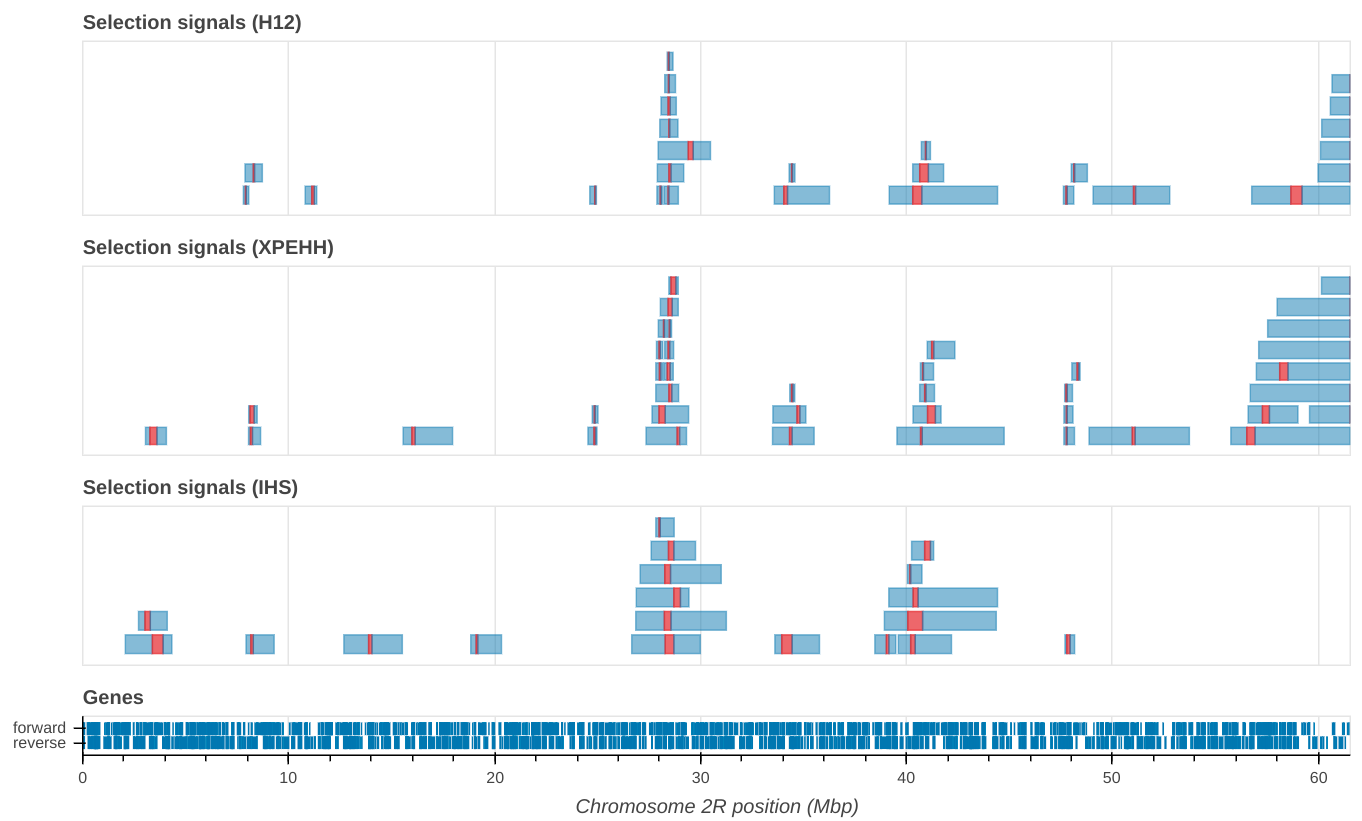
\includegraphics[width=1.1\textwidth,center]{artwork/chapter5/signals_2R.png}
\caption{Selection signals discovered on chromosome arm 2R.
%
Each horizontal bar represents a selection signal.
%
The full width of the bar shows the span of the peak, where the fitted peak model is above 20\% of the peak amplitude.
%
The red region within each bar shows the peak focus, representing the peak center plus a region of uncertainty.
%
}
\label{fig:signals_2R}
\end{figure}


\clearpage
\begin{figure}[h!]
\centering
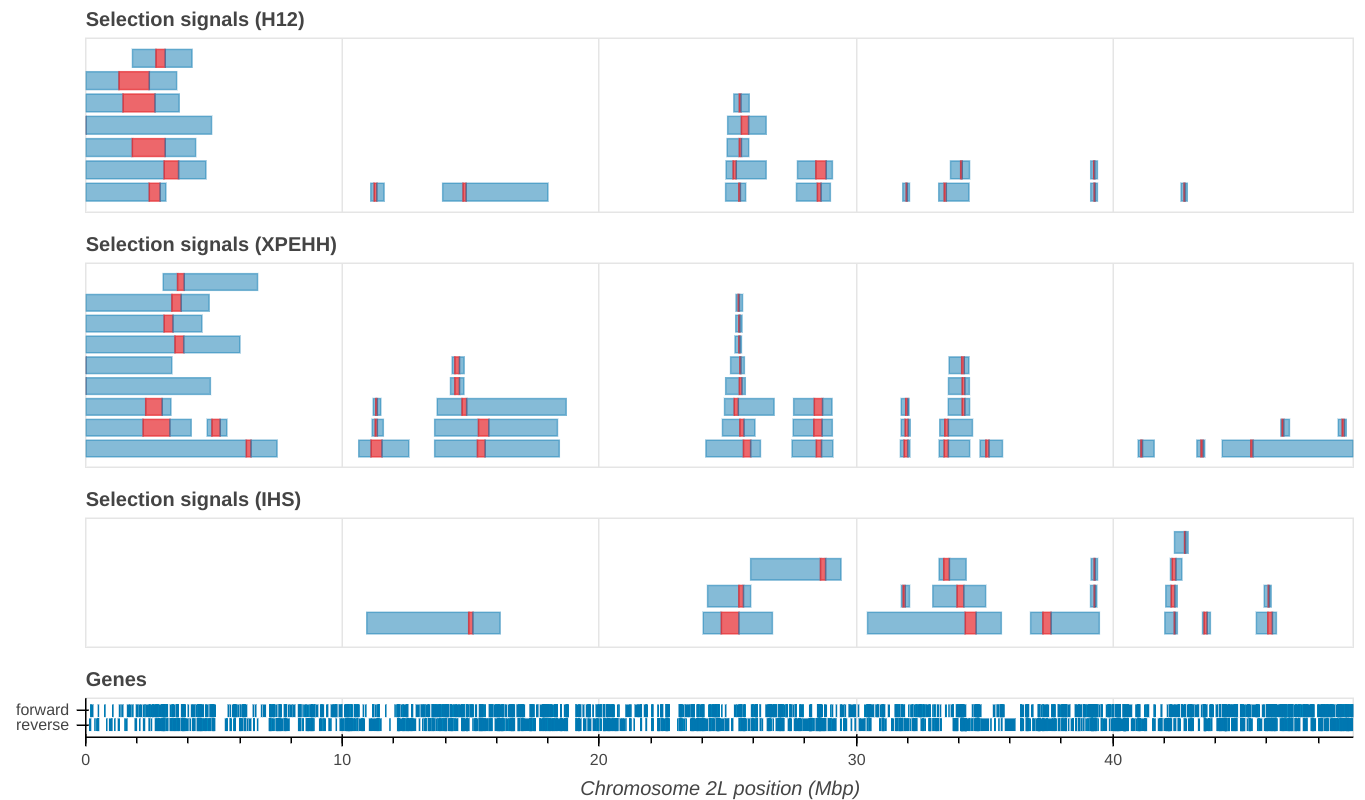
\includegraphics[width=1.1\textwidth,center]{artwork/chapter5/signals_2L.png}
\caption{Selection signals discovered on chromosome arm 2L.
%
See Fig.~\ref{fig:signals_2R} for figure legend.
}
\label{fig:signals_2L}
\end{figure}


\clearpage
\begin{figure}[h!]
\centering
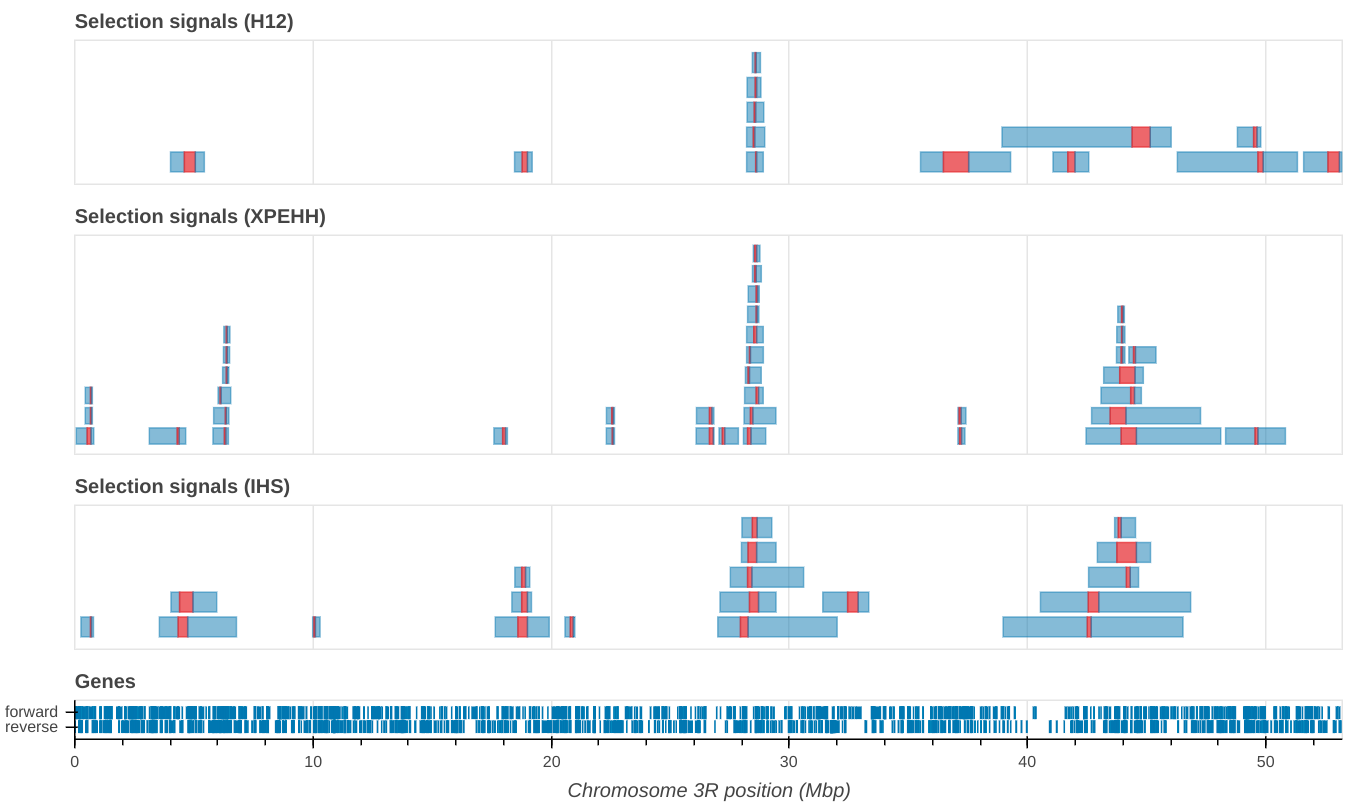
\includegraphics[width=1.1\textwidth,center]{artwork/chapter5/signals_3R.png}
\caption{Selection signals discovered on chromosome arm 3R.
%
See Fig.~\ref{fig:signals_2R} for figure legend.
}
\label{fig:signals_3R}
\end{figure}


\clearpage
\begin{figure}[h!]
\centering
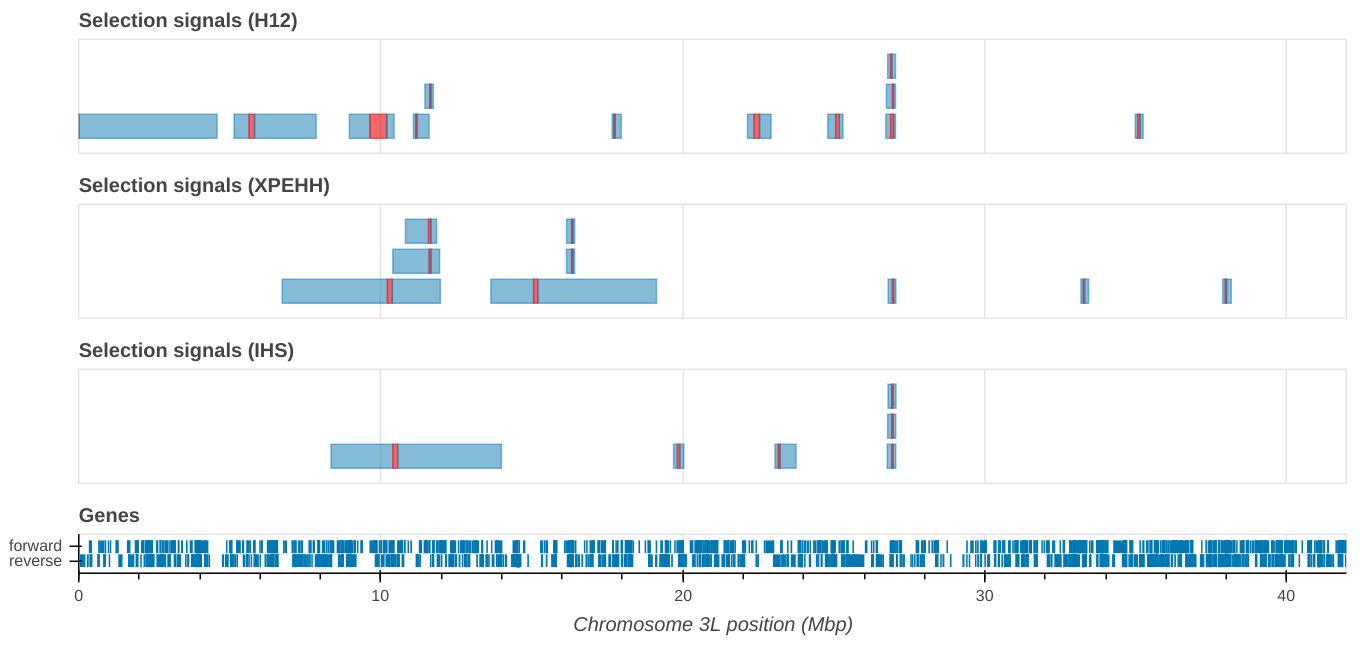
\includegraphics[width=1.1\textwidth,center]{artwork/chapter5/signals_3L.png}
\caption{Selection signals discovered on chromosome arm 3L.
%
See Fig.~\ref{fig:signals_2R} for figure legend.
}
\label{fig:signals_3L}
\end{figure}


\clearpage
\begin{figure}[h!]
\centering
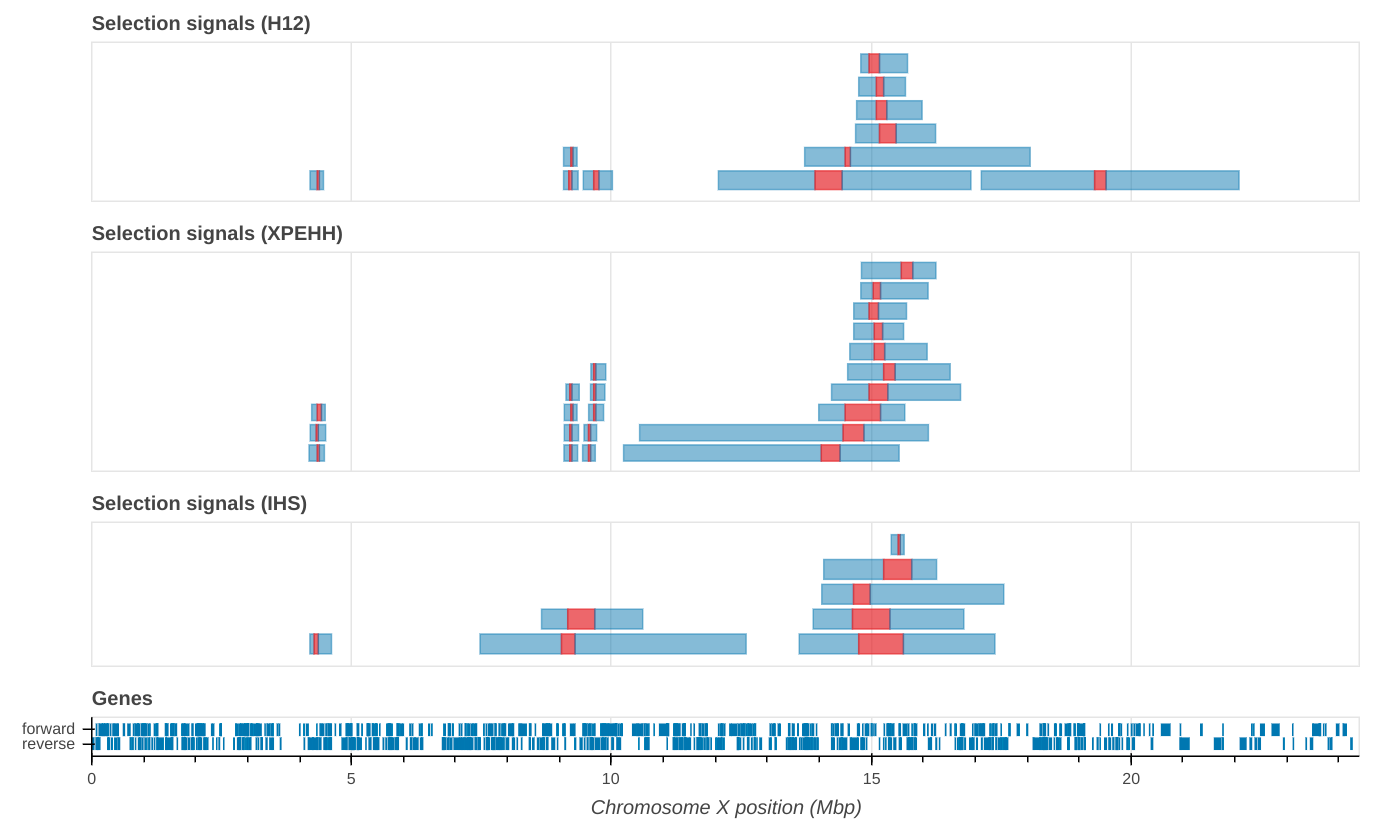
\includegraphics[width=1.1\textwidth,center]{artwork/chapter5/signals_X.png}
\caption{Selection signals discovered on the X chromosome.
%
See Fig.~\ref{fig:signals_2R} for figure legend.
}
\label{fig:signals_X}
\end{figure}


\clearpage
\begin{figure}[h!]
\centering
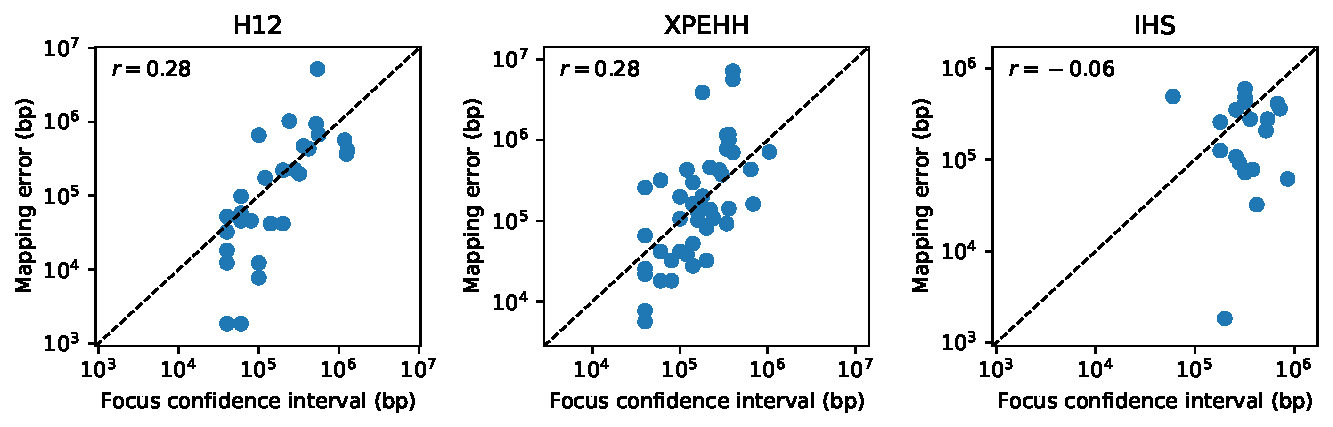
\includegraphics[width=1.1\textwidth,center]{artwork/chapter5/accuracy.pdf}
\caption{Analysis of mapping error and estimated signal focus confidence intervals at known insecticide resistance genes.
%
Each marker represents a selection signal.
%
Each plot compares the confidence interval for the focus of each selection interval, estimated by comparing peak model fits within the vicinity of a signal, and the mapping error, computed as the distance from the fitted peak focus to the known resistance gene.
%
\textit{r} is the Pearson correlation coefficient.
}
\label{fig:accuracy}
\end{figure}


\clearpage
%%%%%%%%%%%%%%%%%%%%%%%%%%%%%%%%%%%%%%%%%%%%%%%%%%%%%%%%%%%%%%%%%%%%%%%%%%%%%%%
%%%%%%%%%%%%%%%%%%%%%%%%%%%%%%%%%%%%%%%%%%%%%%%%%%%%%%%%%%%%%%%%%%%%%%%%%%%%%%%
%%%%%%%%%%%%%%%%%%%%%%%%%%%%%%%%%%%%%%%%%%%%%%%%%%%%%%%%%%%%%%%%%%%%%%%%%%%%%%%
\section{Supplemental tables}\label{sec:ch5-supplemental-tables}


%%%%%%%%%%%%%%%%%%%%%%%%%%%%%%%%%%%%%%%%%%%%%%%%%%%%%%%%%%%%%%%%%%%%%%%%%%%%%%%
\begin{table}[h]
\begin{center}
\begin{threeparttable}
%
\caption{Analysis of sensitivity of selection signal discovery using genes with known insecticide resistance variants.}
%
\label{table:sens}
%
\begin{tabular}{llrrrr}
\toprule
           Gene & Statistic & No. true & No. positive & No. true positive & Sensitivity (\%) \\
\midrule
  \textit{Vgsc} &       H12 &        7 &            7 &                 7 &              100 \\
  \textit{Vgsc} &     XPEHH &        7 &            6 &                 6 &               86 \\
  \textit{Vgsc} &       IHS &        7 &            0 &                 0 &                0 \\
  \textit{Vgsc} &       all &        7 &            7 &                 7 &              100 \\
  \textit{Gaba} &       H12 &        6 &            5 &                 5 &               83 \\
  \textit{Gaba} &     XPEHH &        6 &            5 &                 5 &               83 \\
  \textit{Gaba} &       IHS &        6 &            2 &                 2 &               33 \\
  \textit{Gaba} &       all &        6 &            6 &                 6 &              100 \\
  \textit{Ace1} &       H12 &        2 &            0 &                 0 &                0 \\
  \textit{Ace1} &     XPEHH &        2 &            1 &                 1 &               50 \\
  \textit{Ace1} &       IHS &        2 &            2 &                 2 &              100 \\
  \textit{Ace1} &       all &        2 &            2 &                 2 &              100 \\
 \textit{Gste2} &       H12 &        4 &            5 &                 3 &               75 \\
 \textit{Gste2} &     XPEHH &        4 &            5 &                 3 &               75 \\
 \textit{Gste2} &       IHS &        4 &            5 &                 3 &               75 \\
 \textit{Gste2} &       all &        4 &            6 &                 4 &              100 \\
            all &       H12 &       19 &           17 &                15 &               79 \\
            all &       IHS &       19 &            9 &                 7 &               37 \\
            all &     XPEHH &       19 &           17 &                15 &               79 \\
            all &       all &       19 &           21 &                19 &              100 \\
\bottomrule
\end{tabular}

%
\end{threeparttable}
\end{center}
\end{table}


%%%%%%%%%%%%%%%%%%%%%%%%%%%%%%%%%%%%%%%%%%%%%%%%%%%%%%%%%%%%%%%%%%%%%%%%%%%%%%%
\clearpage
\begin{table}[h]
\begin{center}
\begin{threeparttable}

\caption{Analysis of mapping error using selection signals at known insecticide resistance genes.
%
$N$ = no. of selection signals found overlapping the gene.
%
$ME_n$ = $n^{th}$ percentile of mapping error (distance from signal center to gene) in all selection signals spanning the gene.
%
Within CI = percentage of signals where the gene was within the estimated focus confidence interval.
}

\label{table:acc}

\begin{tabular}{llrrrrrr}
\toprule
            Gene & Statistic & $N$ & $ME_{25}$ & $ME_{50}$ & $ME_{75}$ & Within CI (\%) & Within CI + 50 kb (\%) \\
\midrule
   \textit{Ace1} &       IHS &   2 &       244 &       280 &       316 &             50 &                     50 \\
   \textit{Ace1} &     XPEHH &   1 &        92 &        92 &        92 &            100 &                    100 \\
 \textit{Cyp6p3} &       H12 &   7 &        12 &        32 &        42 &             43 &                     86 \\
 \textit{Cyp6p3} &       IHS &   6 &        77 &       100 &       348 &             67 &                     67 \\
 \textit{Cyp6p3} &     XPEHH &   8 &        31 &        42 &       174 &             62 &                     62 \\
 \textit{Cyp9k1} &       H12 &   6 &        81 &       210 &       552 &             33 &                     50 \\
 \textit{Cyp9k1} &       IHS &   4 &       224 &       320 &       392 &             75 &                     75 \\
 \textit{Cyp9k1} &     XPEHH &  10 &       139 &       162 &       394 &             30 &                     40 \\
   \textit{Gaba} &       H12 &   5 &        46 &        46 &       174 &              0 &                     60 \\
   \textit{Gaba} &       IHS &   2 &       198 &       270 &       342 &             50 &                    100 \\
   \textit{Gaba} &     XPEHH &   8 &        26 &        86 &       133 &             12 &                     88 \\
  \textit{Gste2} &       H12 &   5 &         2 &        18 &        58 &             60 &                     80 \\
  \textit{Gste2} &       IHS &   5 &        78 &       258 &       278 &             60 &                     60 \\
  \textit{Gste2} &     XPEHH &  10 &        26 &        42 &       243 &             30 &                     60 \\
   \textit{Vgsc} &       H12 &   7 &       422 &       472 &       620 &             43 &                     43 \\
   \textit{Vgsc} &     XPEHH &   8 &       757 &      1162 &      4326 &             25 &                     25 \\
             all &       H12 &  30 &        35 &        78 &       427 &             37 &                     63 \\
             all &       IHS &  19 &        85 &       258 &       388 &             63 &                     68 \\
             all &     XPEHH &  45 &        42 &       142 &       428 &             33 &                     56 \\
\bottomrule
\end{tabular}


\end{threeparttable}
\end{center}
\end{table}


\printbibliography[
heading=subbibintoc,
title={References}
]


\end{refsection}
